% !TEX root = ../../main.tex

\section{Results and discussion}

\subsection{Thermal stability}

In order to check if the shaped samples have not undergone bulk
structural changes

The process of shaping did not have any impact on the thermal stability of 
the investigated MOFs, as evidenced by the TGA curves 
(Figure~\ref{fig:ch4:tgacurves}). The primary mass loss occurs 
in a \SI{10}{\degreeCelsius} range for all powder-pellet pairs.
Shaped samples are expected to have a smaller percentage mass loss 
overall due to the addition of the temperature inert alumina. 

\begin{figure}
    \centering
    \begin{subfigure}{0.8\textwidth}
        \parbox[c]{0.1\linewidth}{\caption{}\label{fig:ch4:tgauio66}}%
        \parbox[b]{0.7\linewidth}{%
        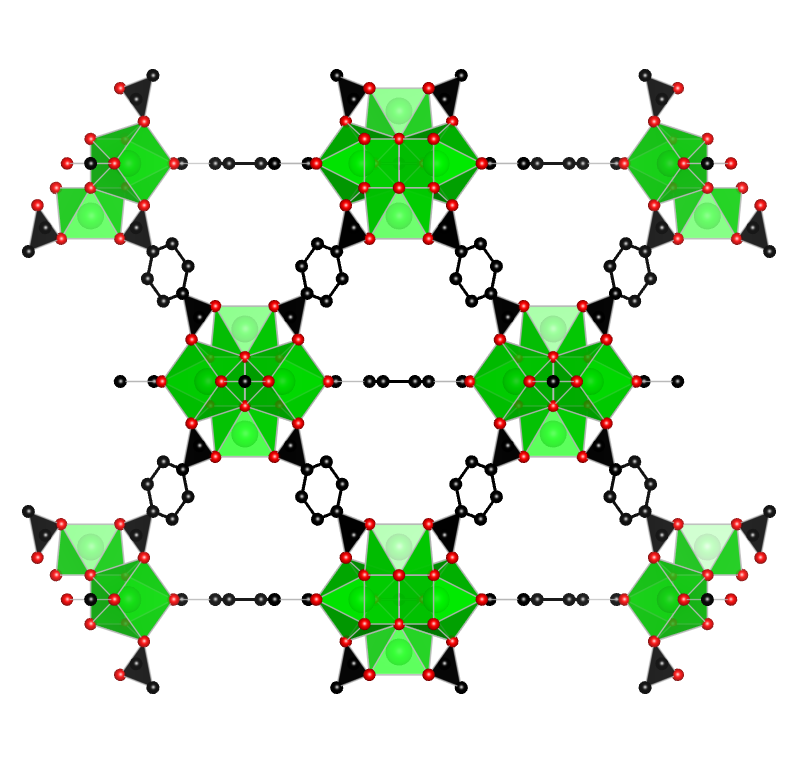
\includegraphics[width=\textwidth]{tga/uio66}%
        }%
    \end{subfigure}

    \begin{subfigure}{0.8\textwidth}
        \parbox[c]{0.1\linewidth}{\caption{}\label{fig:ch4:tgamil100}}%
        \parbox[b]{0.7\linewidth}{%
        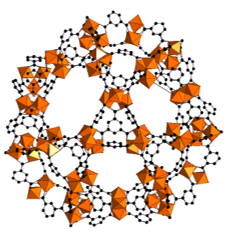
\includegraphics[width=\textwidth]{tga/mil100}%
        }%
    \end{subfigure}

    \begin{subfigure}{0.8\textwidth}
        \parbox[c]{0.1\linewidth}{\caption{}\label{fig:ch4:tgamil127}}%
        \parbox[b]{0.7\linewidth}{%
        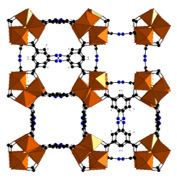
\includegraphics[width=\textwidth]{tga/mil127}%
        }%
    \end{subfigure}
    
    \caption{High resolution TGA curves recoded under argon 
    on (a) UiO-66(Zr), (b) MIL-100(Fe) and (c) MIL-127(Fe)}%
    \label{fig:ch4:tgacurves}

\end{figure}

\subsection{Adsorption isotherms at 77K and room temperature}

Nitrogen sorption isotherms measured at \SI{77}{\kelvin} can be processed to yield
properties such as specific surface area and pore volume for the powders and 
the pellets. The full dataset can be found in Figure~\ref*{fgr:completen277kadsorption}~
in the Supporting Information.

\begin{table}[htbp]
    \centering
    \caption{Properties of the studied powders and pellets}
      \begin{tabular}{lcccc}
      \toprule
      \thead{\textbf{MOF}}
        & \thead{\textbf{form}}
            & \thead{\textbf{BET surface area}}
                & \thead{\textbf{Pore volume}}
                    & \thead{\textbf{Bulk density}} \\
      \midrule
      \multirow{2}{*}{UiO-66(Zr)} & powder & 903 & 0.38 & 0.3192 \\
            & pellet & 619 & 0.24 & 0.4724 \\
      \multirow{2}{*}{MIL-100(Fe)} & powder & 1928 & 0.78 & 0.2165 \\
            & pellet & 1451 & 0.6 & 0.3512 \\
      \multirow{2}{*}{MIL-127(Fe)} & powder & 1400 & x & 0.412 \\
            & pellet & 1266 & 0.49 & 0.526 \\
      \bottomrule
      \end{tabular}\label{tab:propertiestable}
\end{table}%
  
As expected, the specific surface area of the shaped samples is decreased compared to the
corresponding powder. While in the case of MIL-127(Fe) the BET area is only 10\% lower, 
for the MIL-100(Fe) and UiO-66(Zr) materials a larger drop is seen, of 25\% and 31\%,
respectively. 
Another property which can be used to corroborate the effects of shaping is micropore volume,
calculated as the volume of nitrogen adsorbed at a \(p/p^0\) of 0.2. A similar capacity
decrease can be seen here with a 36\%, 23\% and x\% seen in UiO-66(Zr), MIL-100(Fe) and 
MIL-127(Fe) respectively.

\todo{some micropore volumes missing + density}

The decrease in both surface area and micropore volume is too large for it to be a
consequence of the presence of non-porous binder. It is therefore theorised that some 
structure degradation must have occurred in the pelletisation process.

Observation of the physisorption curves sheds light on the further impact of the 
alumina binder on the materials chosen.
The shapes of all isotherms are visually similar, with the pellet ones shifted
downwards due to the aforementioned structure degradation.
In both powders and pellets, the increased uptake after 0.9 \(p/p^0\) is a sign
of condensation in very large pores or voids, which can be attributed to intra-pellet
spaces and crystal agglomeration.
In the MIL-127(Fe) pellets, a narrow hysteresis curve is seen, which closes at a 
\(p/p^0\) of 0.5. This curve corresponds to capillary condensation in a pore size
of around \SI{4}{\nano\metre}. This pore width is too small to be a sign of 
inter-pellet voids and therefore must be a consequence of the shaping process.

\subsection{Water adsorption}

The shape of the water vapour isotherm will be an indication of the hydrophilicity
of the material. By itself, alumina is a hydrophilic substance, with a contact 
angle of \SI{10}{\degree}. It is expected that the addition of the binder will
therefore increase the affinity of the resulting pellet towards water.

Looking at the resulting adsorption measurements one can see the typical downwards
shift of the pellet isotherms resulting from structure degradation. However, changes
in the interaction of the MOF with water do not seem to be highlighted. The low relative
pressure region (\(p/p^0 < 0.3\)) should be particularly indicative of any such 
changes, but an almost complete overlap can be seen in this region.
In particular, the UiO-66(Zr) isotherms have a surprising amount of similarity,
considering the loss of capacity seen in \ce{N2} physisorption and room temperature 
adsorption experiments.

It can be therefore concluded that overall, the addition of alumina has not influenced 
the behaviour towards water for the materials studied. The full water adsorption isotherms
can be found in Figure~\ref*{fgr:completewateradsorption}~, in the Supplementary Information.

\subsection{Room temperature gas adsorption and microcalorimetry}

Combining microcalorimetry with adsorption manometry is a powerful technique which can
give an insight into the strength of the interactions during the adsorption process,
by directly measuring the differential heat. Even though the different contributions 
to the overall enthalpy curve cannot be decoupled from the individual sources, 
such as gas-adsorbent interactions, gas-gas interactions or confinement effects, it 
is well suited for observing the effect of a process or treatment such as shaping
on the properties of a MOF.

A wide variety of probe gasses has been chosen for adsorption at \SI{303}{\kelvin}:
\ce{N2}, \ce{CO}, \ce{CO2}, \ce{CH4}, \ce{C2H6}, \ce{C3H6}, \ce{C3H8} and \ce{C4H10}.
The range of adsorbates chosen allows different effects to be investigated.
The adsorption of saturated hydrocarbons with an increasing carbon number (C1-C4) can be
assumed to be driven strictly by Van-der-Waals forces, due to the shielding effects 
of the hydrogen atoms. Differences in the uptakes of these gasses will point to 
loss of porosity or crystalinity. An assymetric capacity loss with the larger molecules 
will point to size exclusion effects induced by the binder, such as particle coating,
pore filling or pore obstruction.
The other probes have been chosen for their 
individual properties which can shine light on other specific interaction types 
present during the adsorption. 
Carbon monoxide is a slightly dipolar molecule which has the ability to interact with
other charges in the pores. It also can highlight CUS (coordinatively unsaturated sites)
generated through defects, reduction or open metal sites due to its
propensity for \( \pi \) backbonding coordination.
This electron transfer process also can result in complexation with molecular 
orbitals in systems with \( \pi \) bonds such as alkenes and alkynes. Propylene is used 
as a probe gas for this purpose.
Carbon dioxide is a highly quadrupolar molecule which will be strongly adsorbed in 
polar pore environments. Changes in the adsorption behaviour of \ce{CO2} will shed 
light on such surface changes and can even be used as a predictor of 
hydrophobicity~\cite{chanutScreeningEffectWater2017}.
Finally, \ce{N2} is a staple adsorbent for material characterisation when used at
\SI{77}{\kelvin}. The molecule is a slight quadrupole and has also been shown to 
chelate to some transitional metals in an analogue fashion to \ce{CO}.

To eliminate the influence of kinetic and diffusion effects on the experiments,
care has been taken to allow time for complete equilibration of both pressure
and calorimeter signal.

After collecting the combined isotherm enthalpy data, three indicators have been chosen
to best represent the effects of shaping: initial enthalpy of adsorption, initial 
Henry constant and maximum capacity. These numeric performance indicators have been
calculated programmatically in Python using a specially developed high throughput
package.
The initial enthalpy of adsorption extrapolated at zero coverage is a measure of the 
interaction with highest energetic sites on the MOF surface. Conversely, the 
\(K_H\) obtained by applying the linear Henry model at the lowest loading points
is also an indication of adsorption in the pores before any 
layering or adsorbate-adsorbate interaction comes into effect. The \(K_H\) was 
calculated by fitting the virial adsorption model (Equation~\ref{eqn:virial})
to the isotherm.
The last indicator, maximum capacity, was taken as the loading attained when 
the isotherm reached a plateau. In the case of probes where the plateau was outside 
the range of pressure of the instrumentation (>\SI{50}{\bar}), the loading at the 
highest available pressure was considered as a suitable approximation.
The three KPIs (key performance indicators) have then been compared side by 
side on both the powder and shaped samples. 

\begin{equation}
    \label{eqn:virial}
    \ln{\frac{n}{P}} = \ln{K_H} + An + Bn^2 \cdots
\end{equation}

The complete dataset of adsorption isotherms, in the basis of both mass and volume 
can be found in the Supplementary Information (Figures~\ref*{fgr:calouio66}~,
\ref*{fgr:calomil100}~~and~\ref*{fgr:calomil127}~).

\subsubsection{UiO-66(Zr)}

A visual inspection of the enthalpy curves on UiO-66(Zr) show it to have a 
relatively homogenous surface, with flat profiles being common.

The KPI graphs show very similar values for both Henry's constant and initial 
enthalpy of adsorption. It is therefore apparent that the shaping process did not 
change the interaction of the adsorbate with the MOF surface.

The maximum capacity graphs show a more interesting trend. When using small adsorbates
such as \ce{N2}, \ce{CO2} and \ce{CH4}, the shaped samples have a similar performance 
on a mass basis and, due to the densification process, better capacities on a volume
basis. Starting with ethane, the maximum capacity starts to decrease, with the performance
worsening with increasing molecule size. On hydrocarbons with a carbon number of 3 and 4,
both mass basis and volume basis capacity is decreased compared to the original powder.
Carbon monoxide is an apparent outlier to this trend, with a decreased maximum capacity
and a small molecular size. 
This size exclusion effect could be explained by the coating of crystal surfaces with 
the alumina binder.
It could be argued that instead of size exclusion, the decrease is due to
a decrease in pore volume, and that the isotherms of the low molecular 
weight gasses will diverge at higher pressures as the pores are filled. 
A counterargument for this hypothesis is that on \ce{CO} a divergence 
is observed while the isotherm is still in the Henry's region and in the 
case of \ce{CO2}, the plateau is reached with no differences between the 
powder and the pellet.

Overall, the shaping performance of UiO-66(Zr) is 
reasonable, as long as only small adsorbates are used.

\begin{figure}
    \centering
    \begin{subfigure}{0.8\textwidth}
        \parbox[c]{0.1\linewidth}{\caption{}\label{fig:analysisuio66henry}}%
        \parbox[b]{0.7\linewidth}{%
        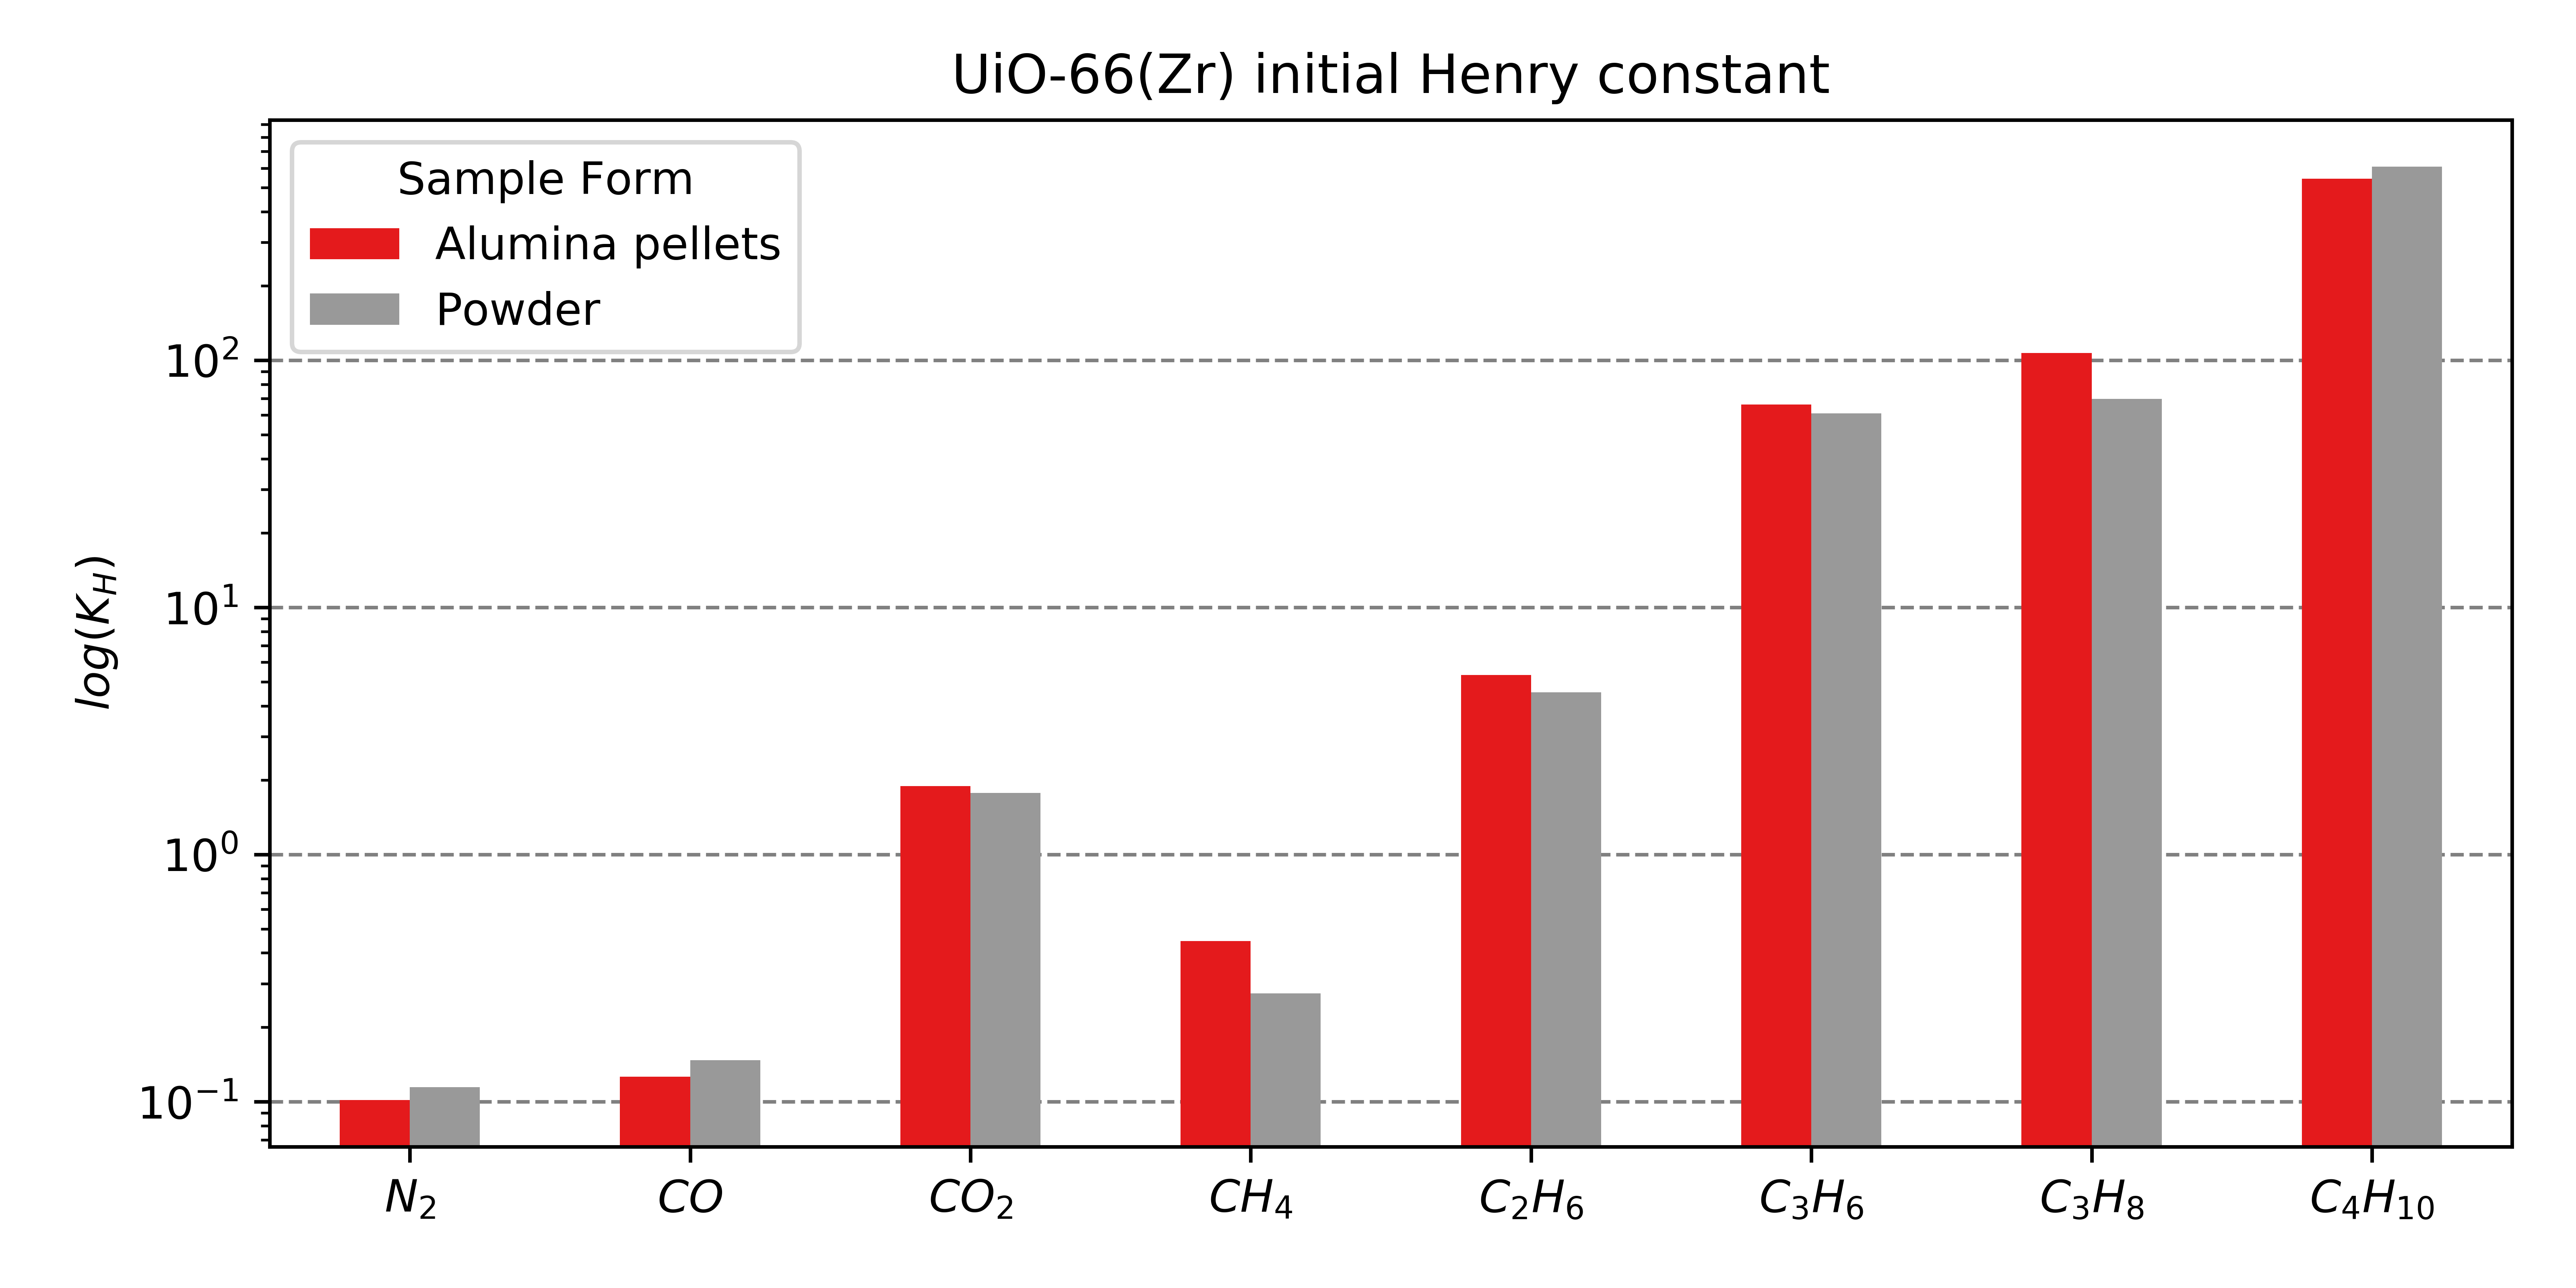
\includegraphics[width=\textwidth]{UiO-66(Zr)-henry-distribution}%
        }%
    \end{subfigure}

    \begin{subfigure}{0.8\textwidth}
        \parbox[c]{0.1\linewidth}{\caption{}\label{fig:analysisuio66enth}}%
        \parbox[b]{0.7\linewidth}{%
        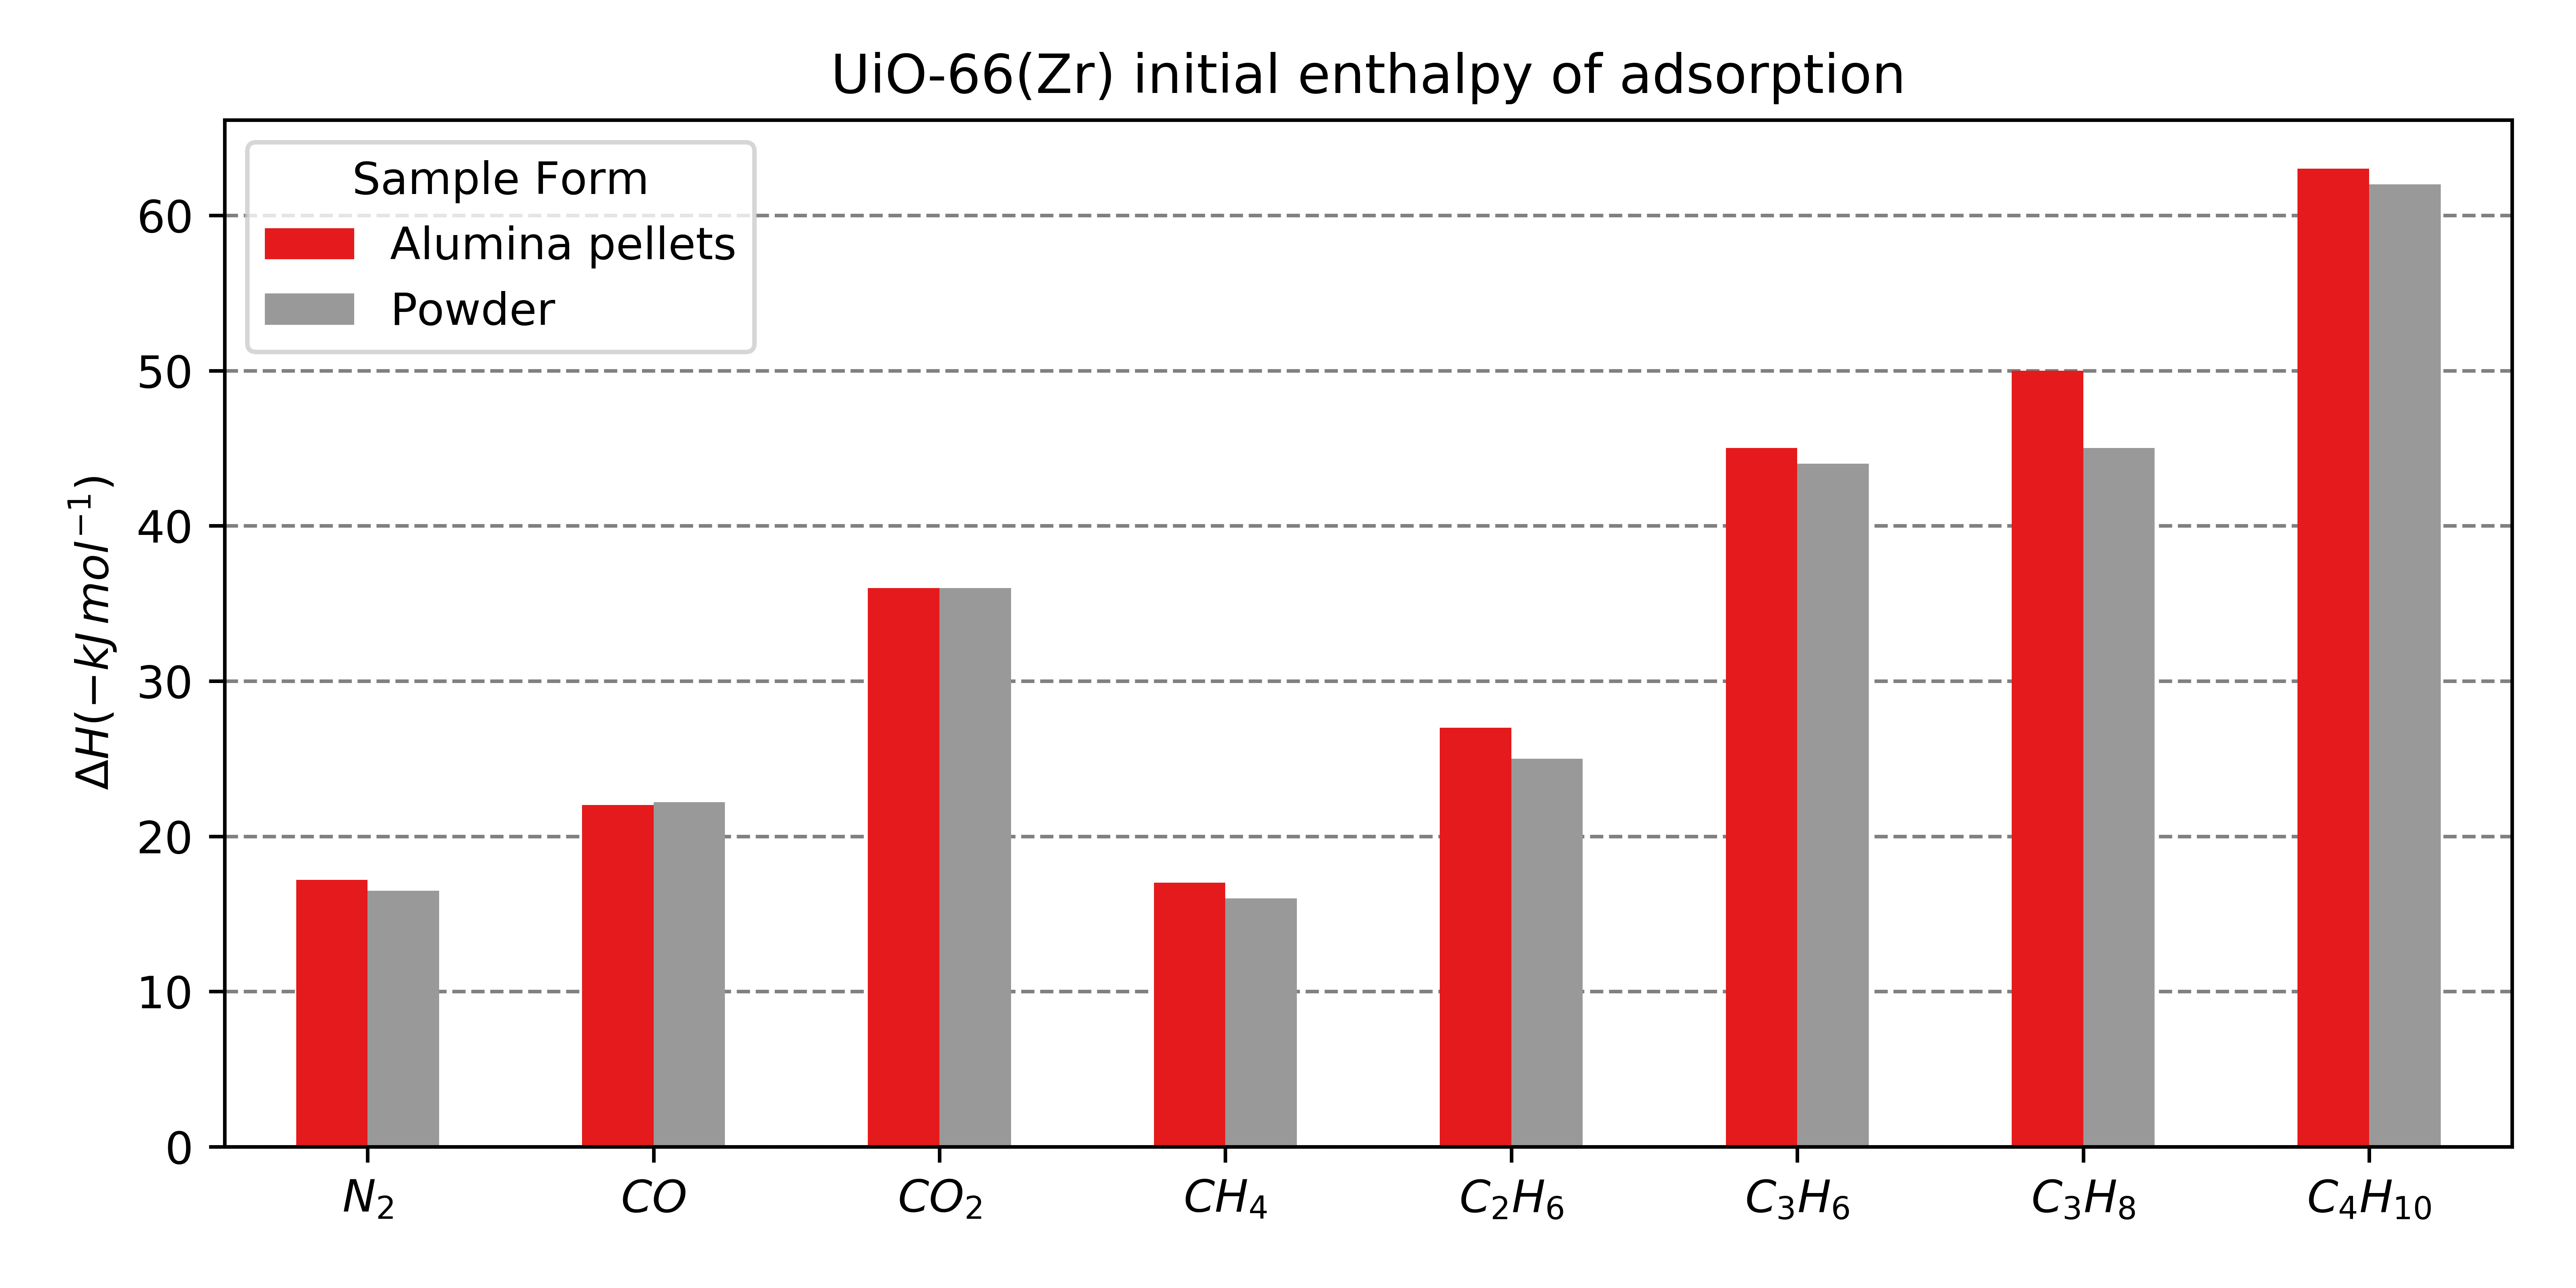
\includegraphics[width=\textwidth]{UiO-66(Zr)-enthalpy-distribution}%
        }%
    \end{subfigure}

    \begin{subfigure}{0.8\textwidth}
        \parbox[c]{0.1\linewidth}{\caption{}\label{fig:analysisuio66basis}}%
        \parbox[b]{0.7\linewidth}{%
        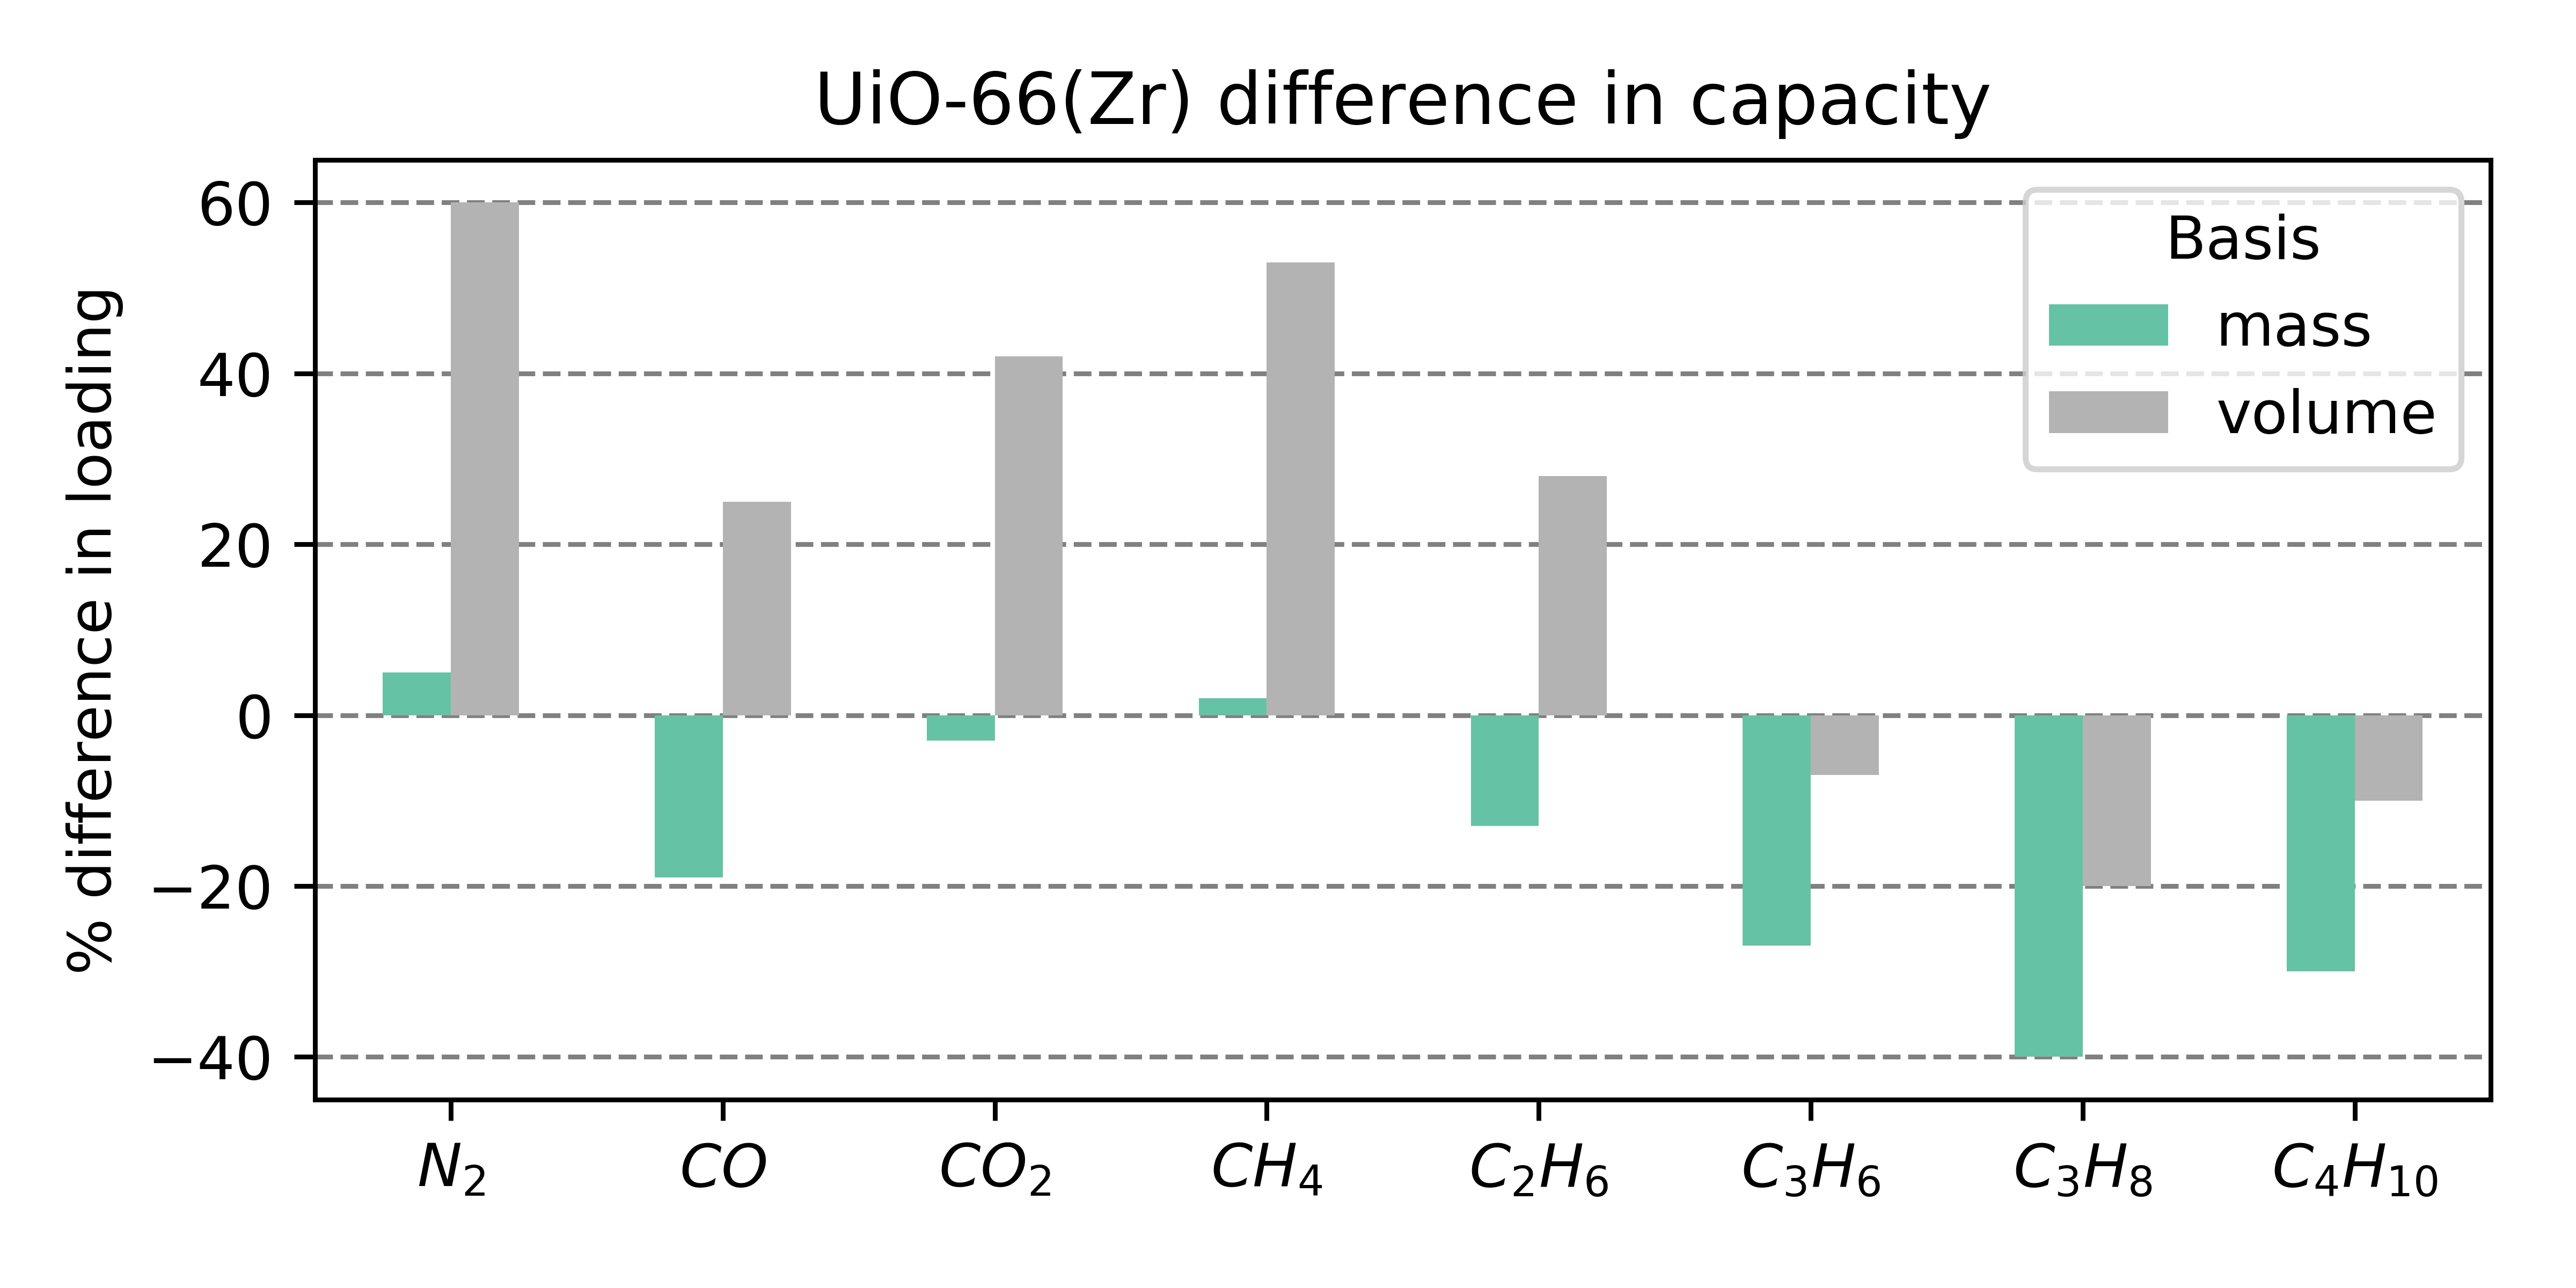
\includegraphics[width=\textwidth]{UiO-66(Zr)-mass-volume}%
        }%
    \end{subfigure}
    
    \caption{UiO-66(Zr) analysis}%
    \label{fig:analysisuio66}
\end{figure}

\subsubsection{MIL-100(Fe)}

The enthalpy profiles on MIL-100(Fe) are less homogenous than the ones on UiO-66(Zr). 
Some effects can
be seen with probes which can interact with the partially reduced Fe(II) atom, such as 
carbon monoxide and propylene. 
Indeed, when comparing both the initial Henry constants and enthalpy of adsorption,
for \ce{CO} and \ce{C3H6}, these are higher than the values obtained on UiO-66(Zr).
With initial enthalpy of adsorption for \ce{CO} of around \SI{45}{\kilo\joule\per\mol},
the value falls into the range of previous~\cite{yoonControlledReducibilityMetalOrganic2010}
results for interactions with such Fe(II) CUS.

Comparing the powder and shaped variants, there are no 
apparent differences between the two. The only discrepancy, which can be seen on the 
nitrogen \(K_{H, init}\) follows as a result of an ill-fitting virial parameter,
and can be assumed an error after observing the isotherm overlap directly. It could be 
theorised that by activation at a higher temperature (\SI{250}{\degreeCelsius}),
the percentage of iron trimers which would undergo reduction will increase and 
a larger adsorption enthalpy could be observed. However, the
activation temperature was chosen to maintain comparability with a previous 
study~\cite{chanutObservingEffectsShaping2016}.

The maximum loading differences of the MIL-100(Fe) show a very homogenous distribution.
On all probes tested, a fixed capacity loss of between 10-20\% can be seen on a mass 
basis. However, the increase in density afforded by the compression during pelletisation
leads to a compensation in performance as can be seen in Figure~\ref{fig:analysismil100basis}.

We can conclude that MIL-100(Fe) is almost unaffected by alumina shaping. A slight loss
in maximum capacity on a mass basis is compensated by a pronounced densification, 
which is desirable in an industrial setting.

\begin{figure}
    \centering
    \begin{subfigure}{0.8\textwidth}
        \parbox[c]{0.1\linewidth}{\caption{}\label{fig:analysismil100henry}}%
        \parbox[b]{0.7\linewidth}{%
        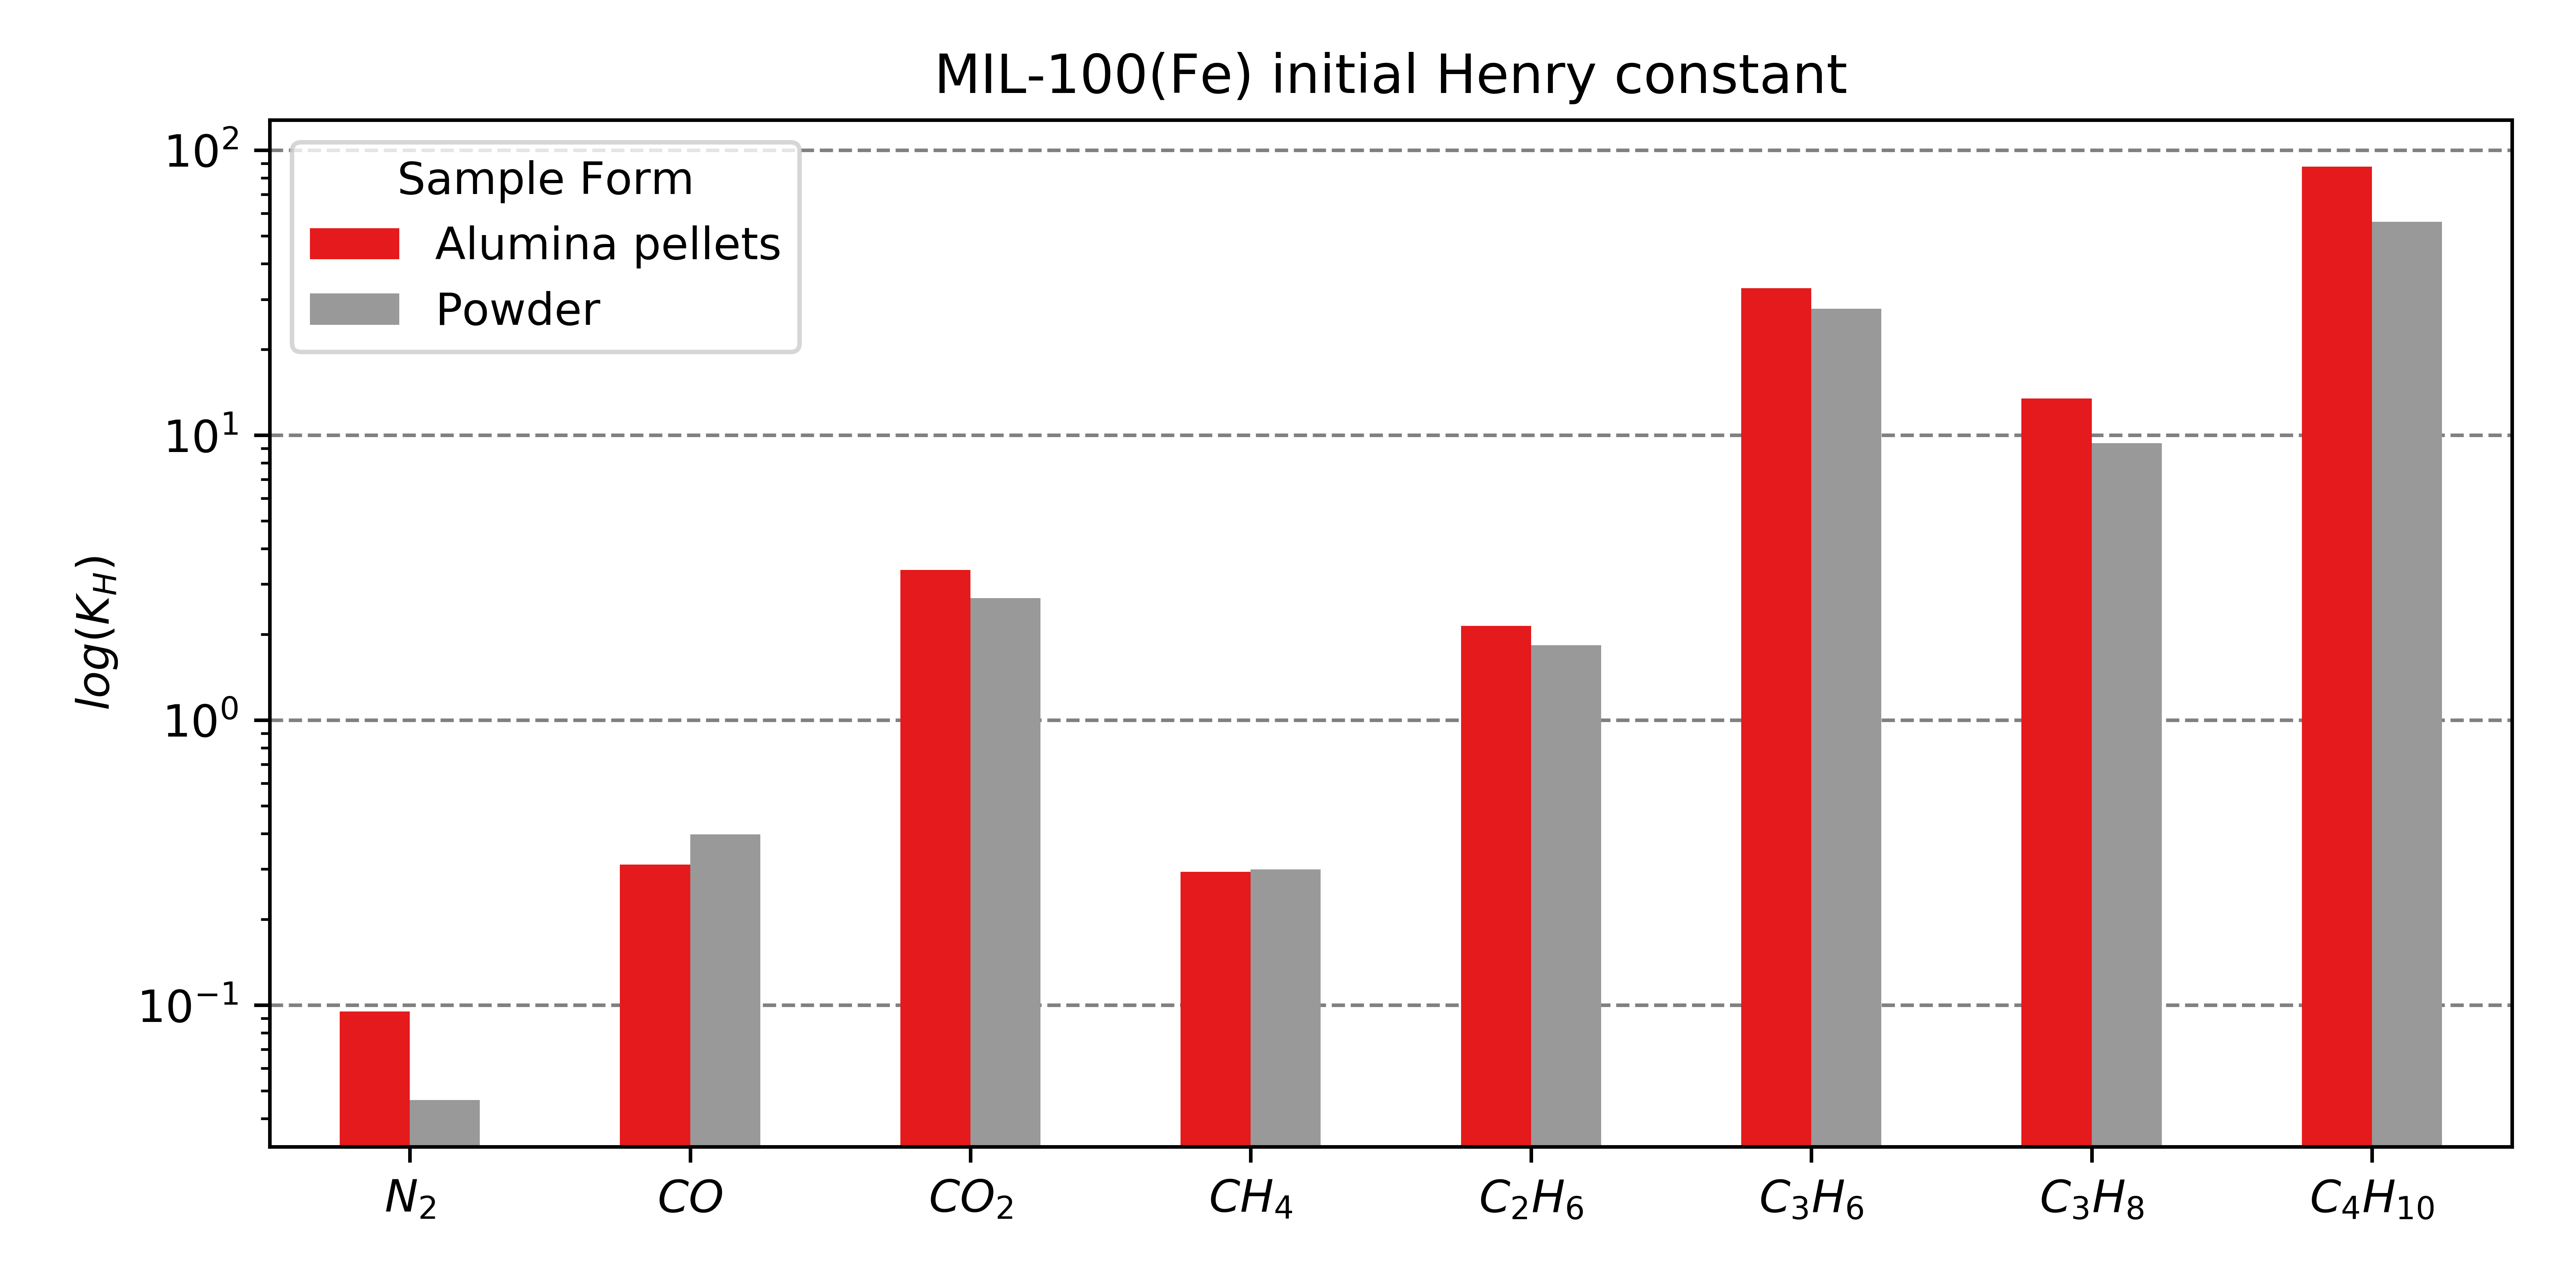
\includegraphics[width=\textwidth]{MIL-100(Fe)-henry-distribution}%
        }%
    \end{subfigure}

    \begin{subfigure}{0.8\textwidth}
        \parbox[c]{0.1\linewidth}{\caption{}\label{fig:analysismil100enth}}%
        \parbox[b]{0.7\linewidth}{%
        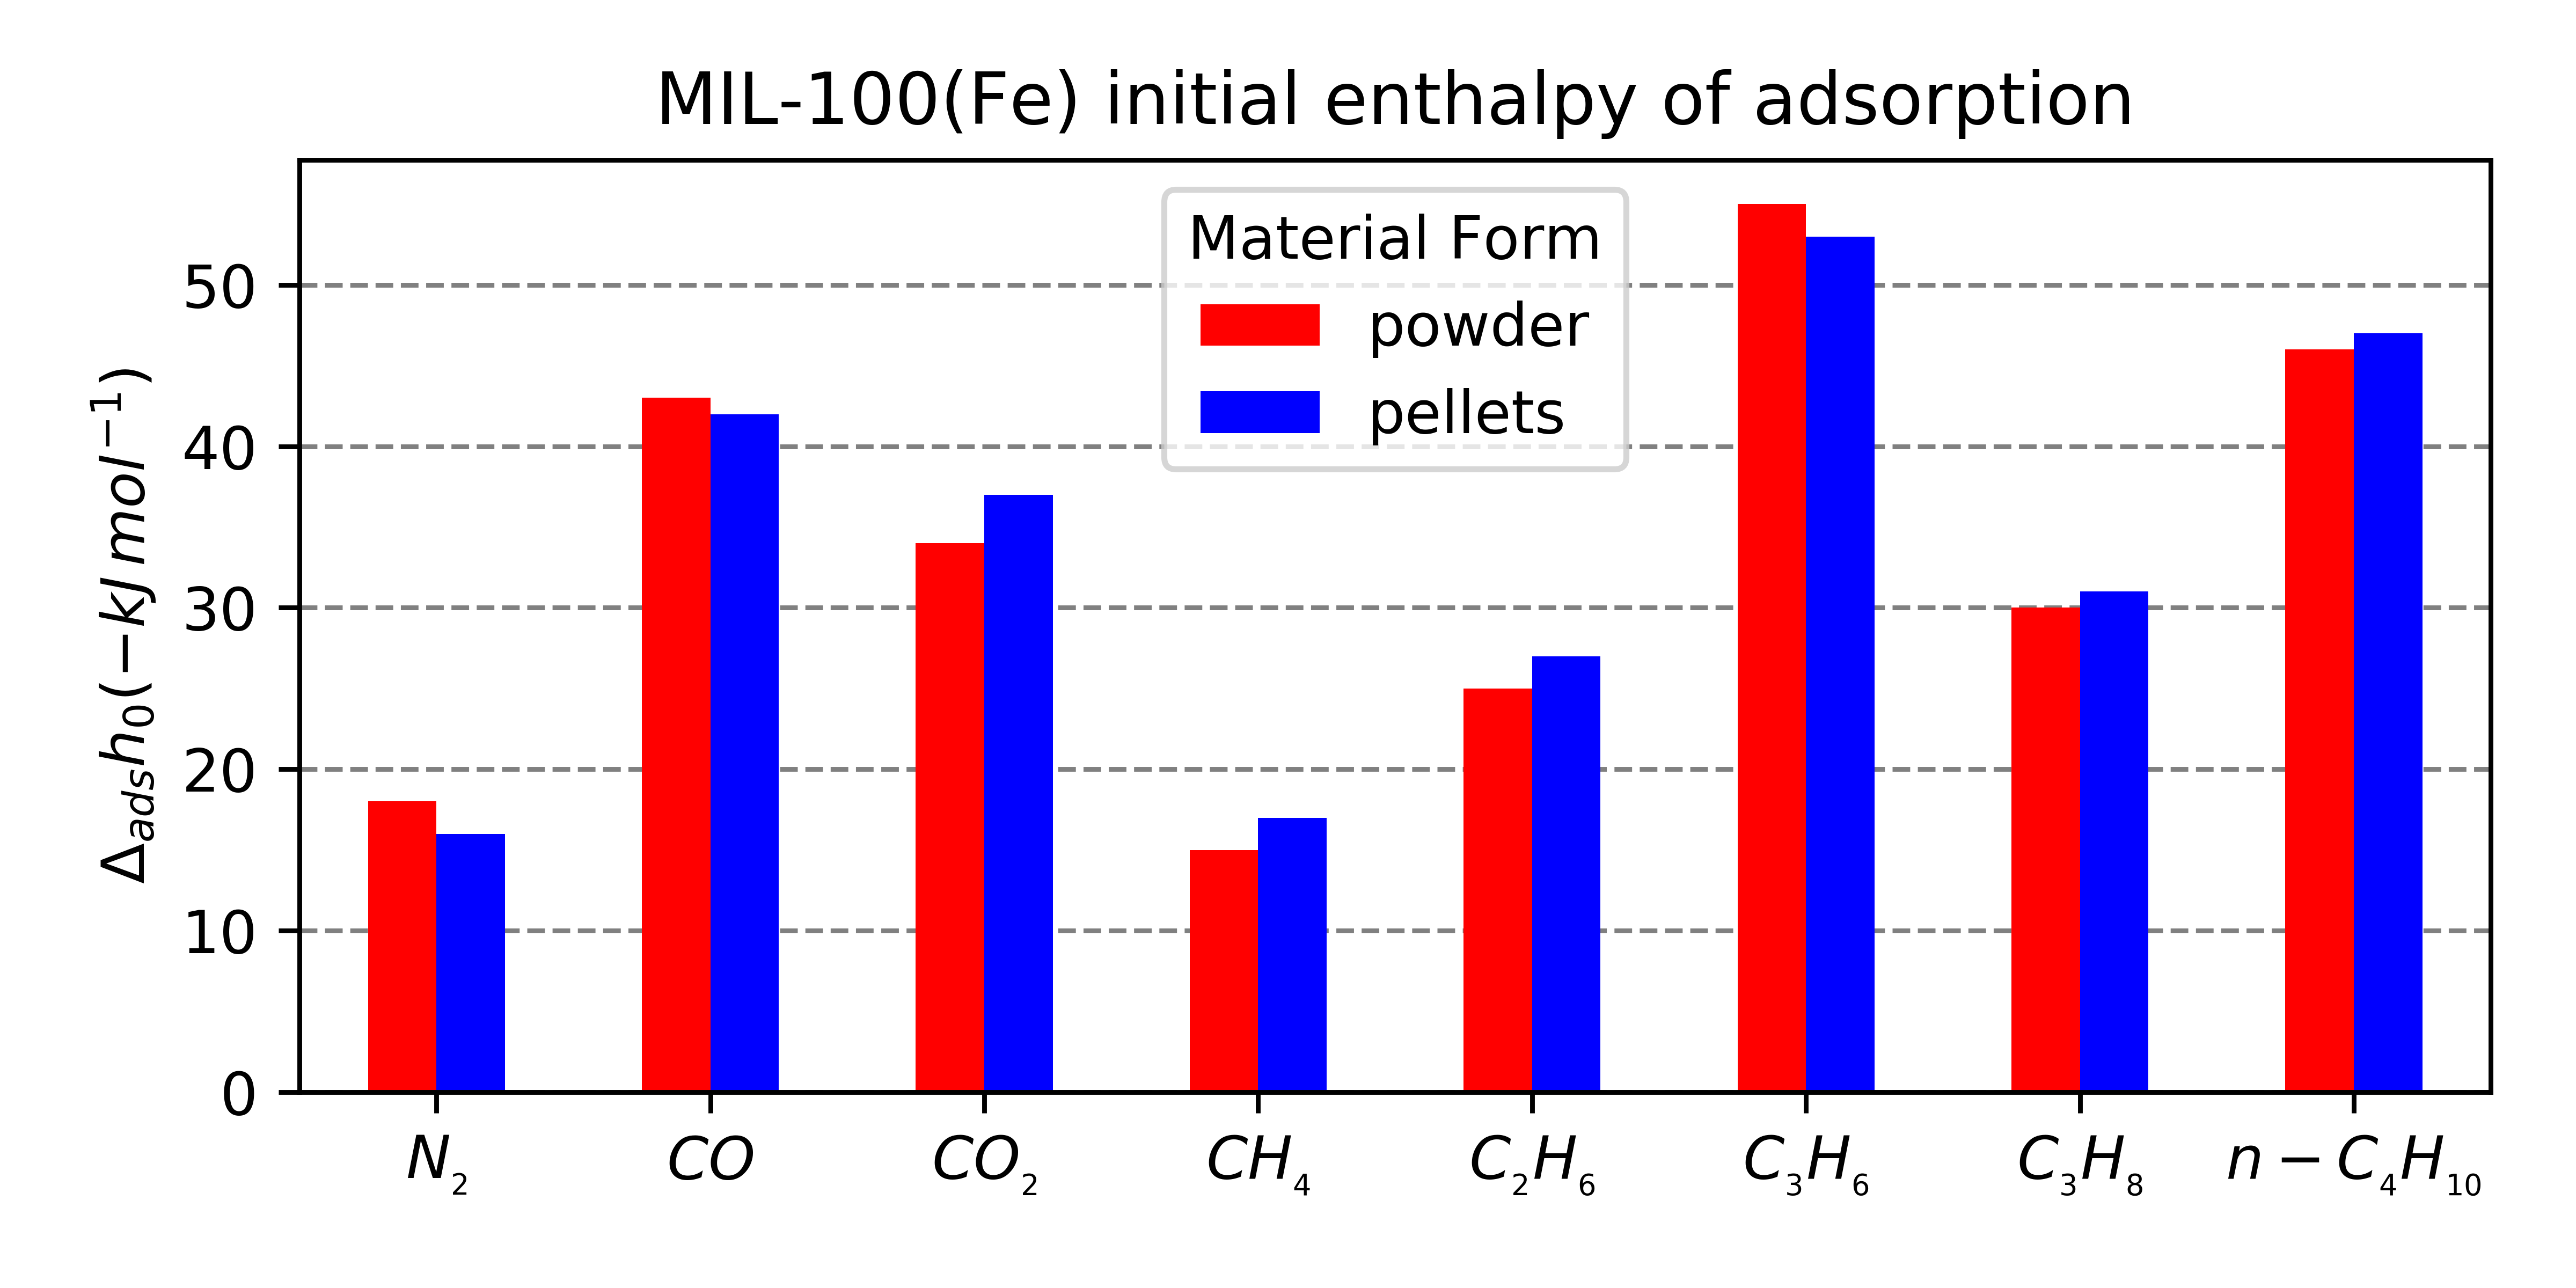
\includegraphics[width=\textwidth]{MIL-100(Fe)-enthalpy-distribution}%
        }%
    \end{subfigure}

    \begin{subfigure}{0.8\textwidth}
        \parbox[c]{0.1\linewidth}{\caption{}\label{fig:analysismil100basis}}%
        \parbox[b]{0.7\linewidth}{%
        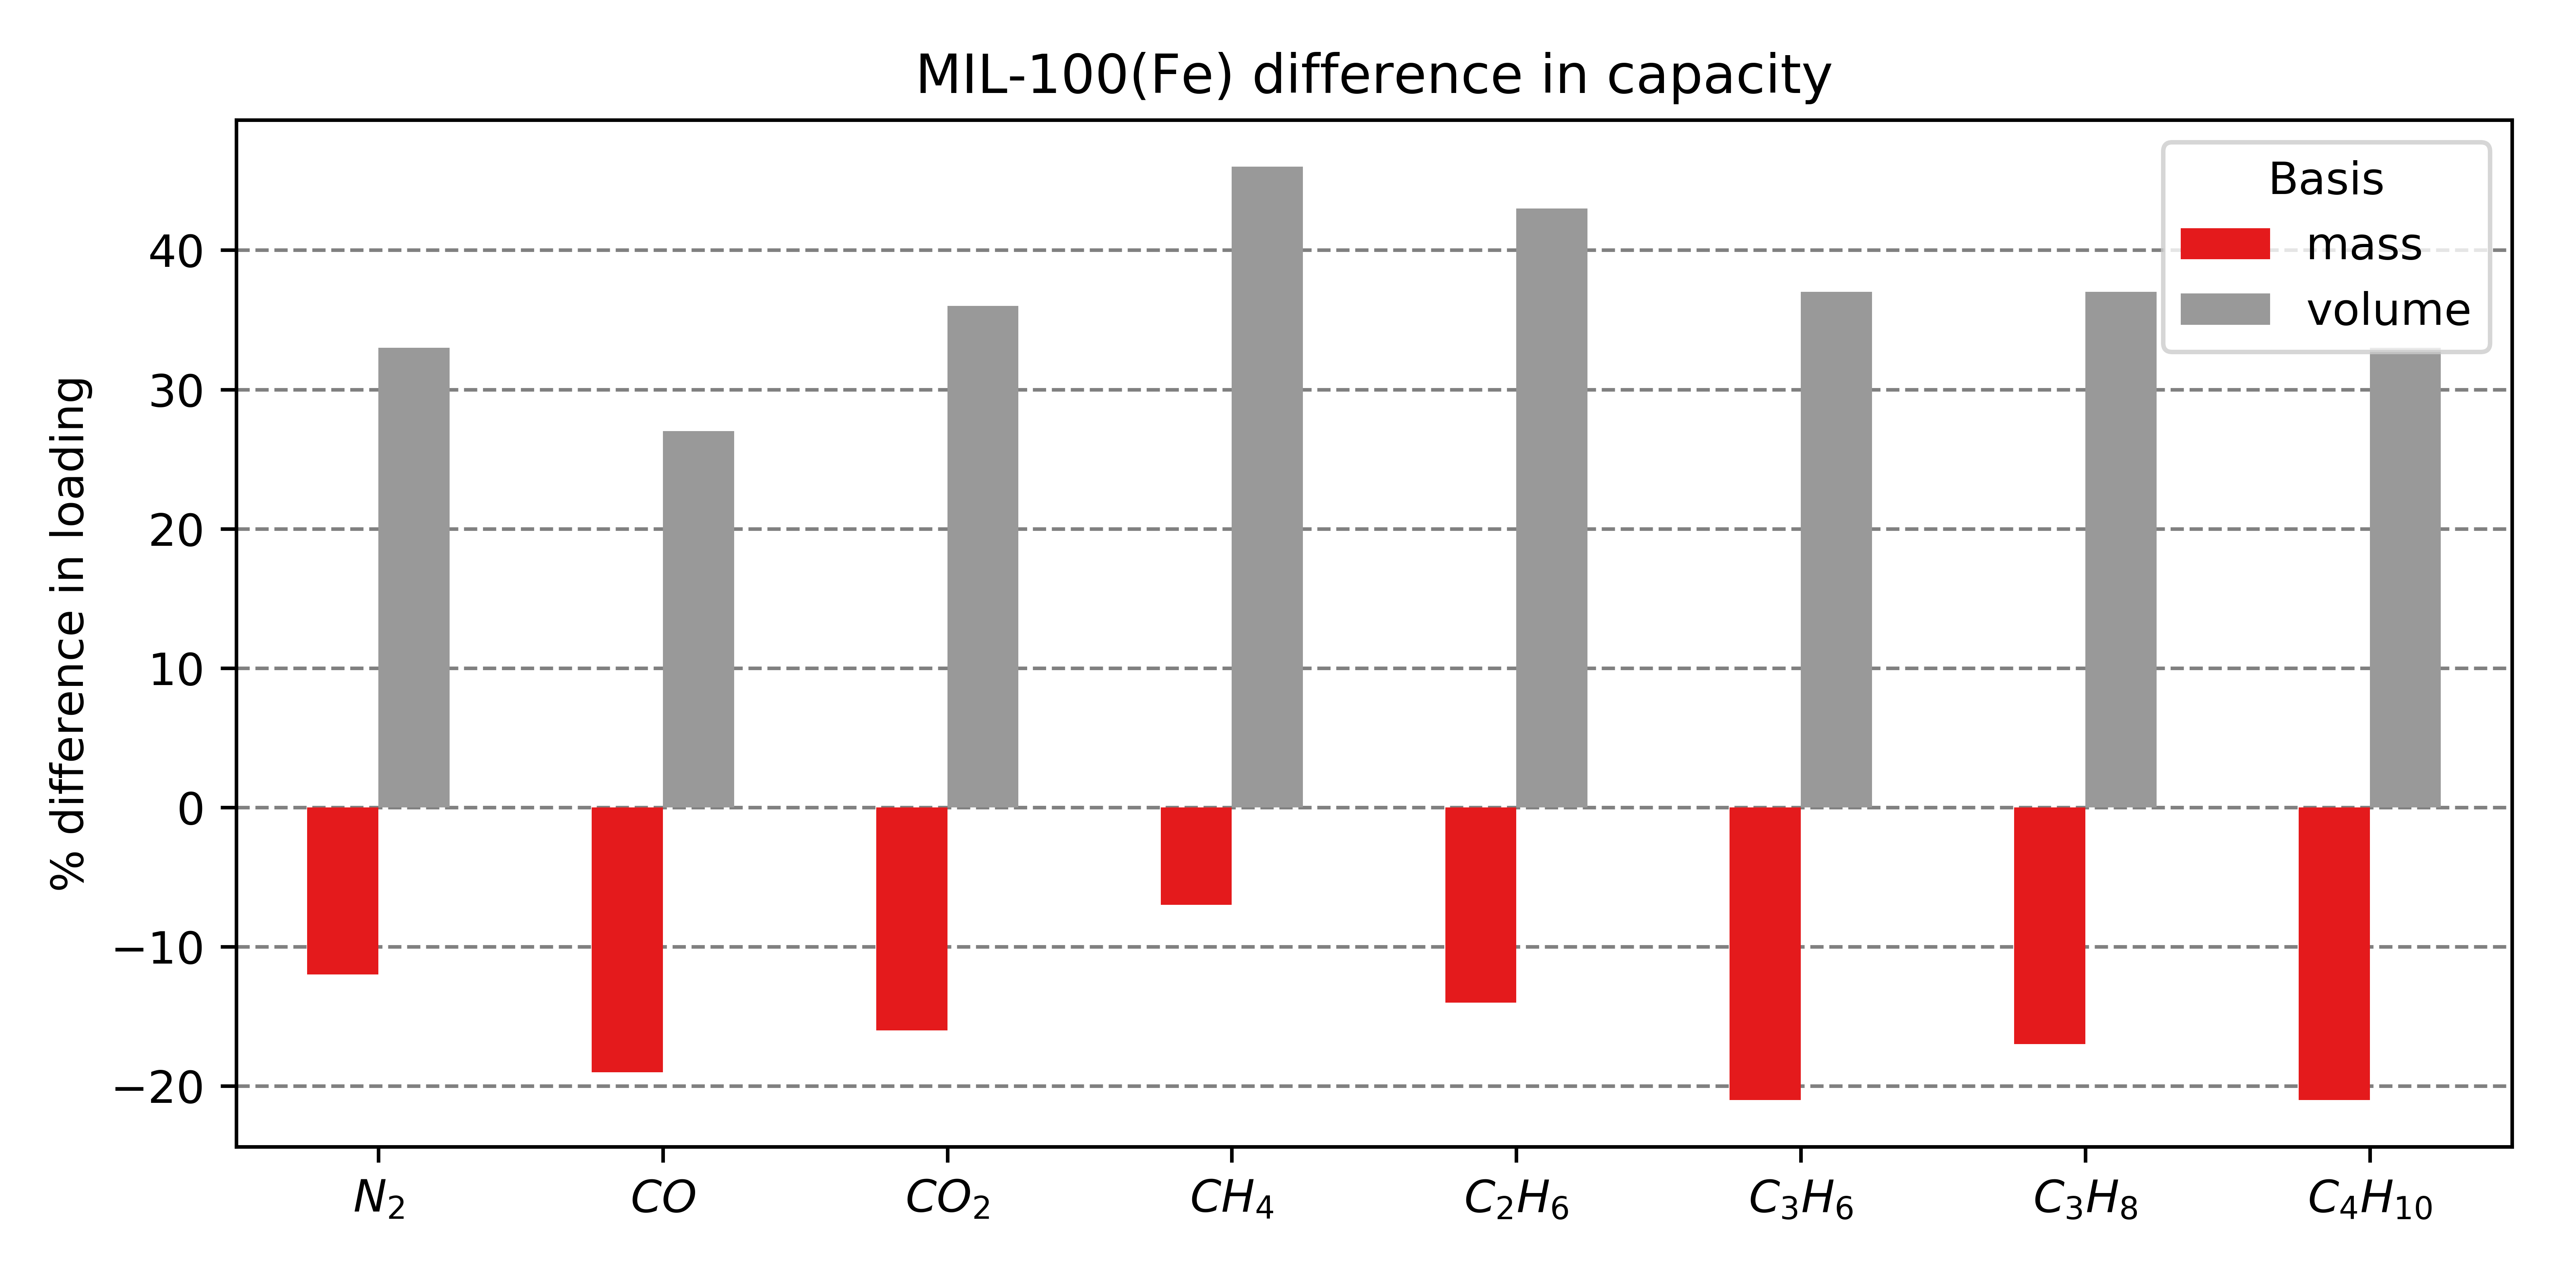
\includegraphics[width=\textwidth]{MIL-100(Fe)-mass-volume}%
        }%
    \end{subfigure}
    
    \caption{MIL-100(Fe) analysis}%
    \label{fig:analysismil100}
\end{figure}

\subsubsection{MIL-127(Fe)}

The isotherms on MIL-127(Fe) show similar behaviour as the MIL-100(Fe) material,
although with a sharper uptake as a result of the smaller pores. Enthalpy 
profiles are also influenced by the similar interactions with the iron 
trimers leading to higher initial heats of adsorption on \ce{CO} and \ce{C3H6}.
An unexpected increase in the heat of adsorption is seen with 
butane adsorption (Figure~\ref{fgr:mil127c4h10ads}). Due to the dual pore 
type in the MIL-127(Fe) structure,
it is likely that adsorption first commences in the small (\( \sim \)\SI{6}{\angstrom})
channels and then, at higher pressures, intrusion into the larger cage-type
pores is possible through the narrow apertures of \( \sim \)\SI{3}{\angstrom}. 
The confined cages have an increased interaction with the molecule which 
leads to the higher enthalpy values.

When observing the comparison between the powder and the pellet variant, a large
difference in the initial \(K_H\) on \ce{CO} stands out as the only major change.
The value of the initial enthalpy of adsorption does not follow the same pattern.
However, visual inspection of the isotherm (Figure~\ref{fgr:mil127coads})
and the enthalpy curve shows that the energy of adsorption corresponding to
interactions with the more active sites is maintained for a larger pressure 
range. This points to the higher preponderence of such sites in the powder
variant. A similar offset can be seen in the propylene enthalpy at very low
pressures, but this is not reflected in the shape of the isotherm. The weaker 
complexation strength and the larger size of the molecule likely limits the effect 
seen in the carbon monoxide isotherm. As for the underlying reason behind the 
isotherm divergence, it could be that the alumina binder acts as a protector against the 
generation of iron(II) during thermal activation.
No other differences are seen between the two forms on either Henry constant and
initial enthalpy of adsorption.

\begin{figure}[ht]
    \begin{subfigure}{0.5\textwidth}
        \includegraphics[width=\textwidth]{calo/MIL-127(Fe)/c4h10-mass-basis-log-iso}
        \caption{\ce{C4H10} isotherms on MIL-127(Fe)}%
        \label{fgr:mil127c4h10ads}
    \end{subfigure}
    \begin{subfigure}{0.5\textwidth}
        \includegraphics[width=\textwidth]{calo/MIL-127(Fe)/co-mass-basis-iso}
        \caption{CO isotherms on MIL-127(Fe)}%
        \label{fgr:mil127coads}
    \end{subfigure}%
    \label{fgr:mil127isotherms}
\end{figure}

The capacity comparison in Figure~\ref{fig:analysismil127basis} paints an interesting 
picture. For most probes there is no change in maximum loading showing that there is no
structure degradation or pore filling. Two outliers are apparent: carbon monoxide and 
butane. The decrease in capacity on \ce{CO} can be explained through the 
aforementioned changes in active site prevalence. The drop in butane cannot be a 
consequence of the same effect as there is a perfect overlap in the enthalpy curves.
Therefore it best explained through a size exclusion effect as seen on UiO-66(Zr).

Overall, MIL-127(Fe) shows excellent performance when undergoing alumina shaping, with 
almost no capacity loss, as long as the adsorbent is not carbon monoxide or butane, 
where specific effects come into play.

\begin{figure}
    \centering
    \begin{subfigure}{0.8\textwidth}
        \parbox[c]{0.1\linewidth}{\caption{}\label{fig:analysismil127henry}}%
        \parbox[b]{0.7\linewidth}{%
        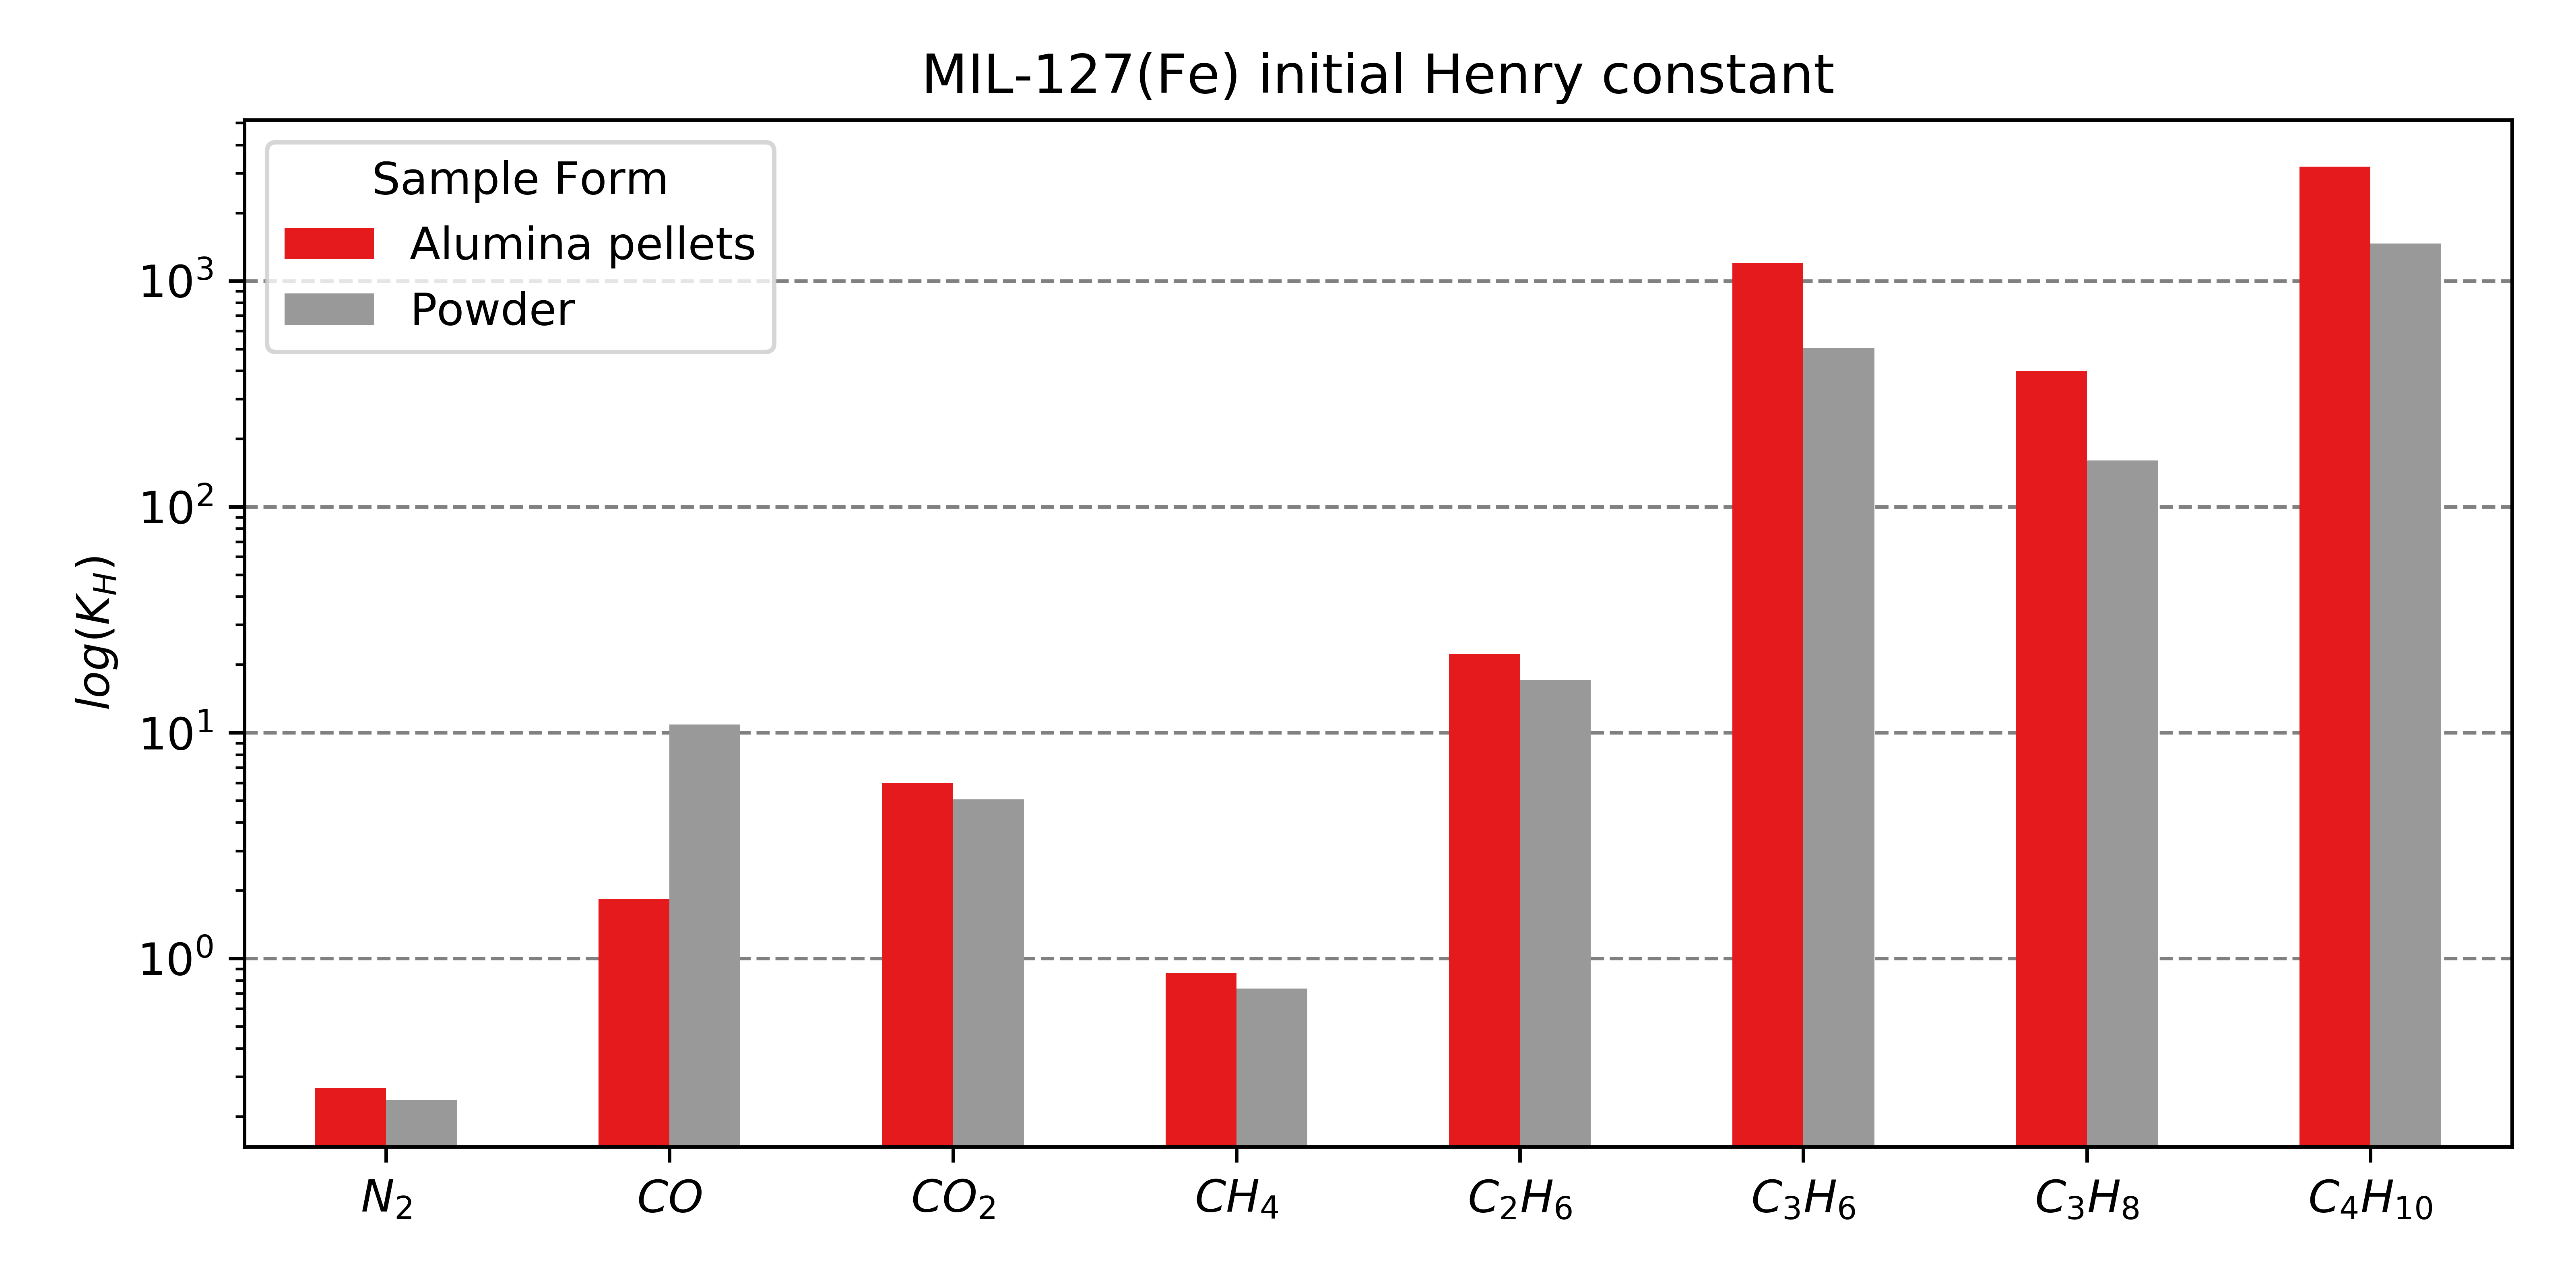
\includegraphics[width=\textwidth]{MIL-127(Fe)-henry-distribution}%
        }%
    \end{subfigure}
    
    \begin{subfigure}{0.8\textwidth}
        \parbox[c]{0.1\linewidth}{\caption{}\label{fig:analysismil127enth}}%
        \parbox[b]{0.7\linewidth}{%
        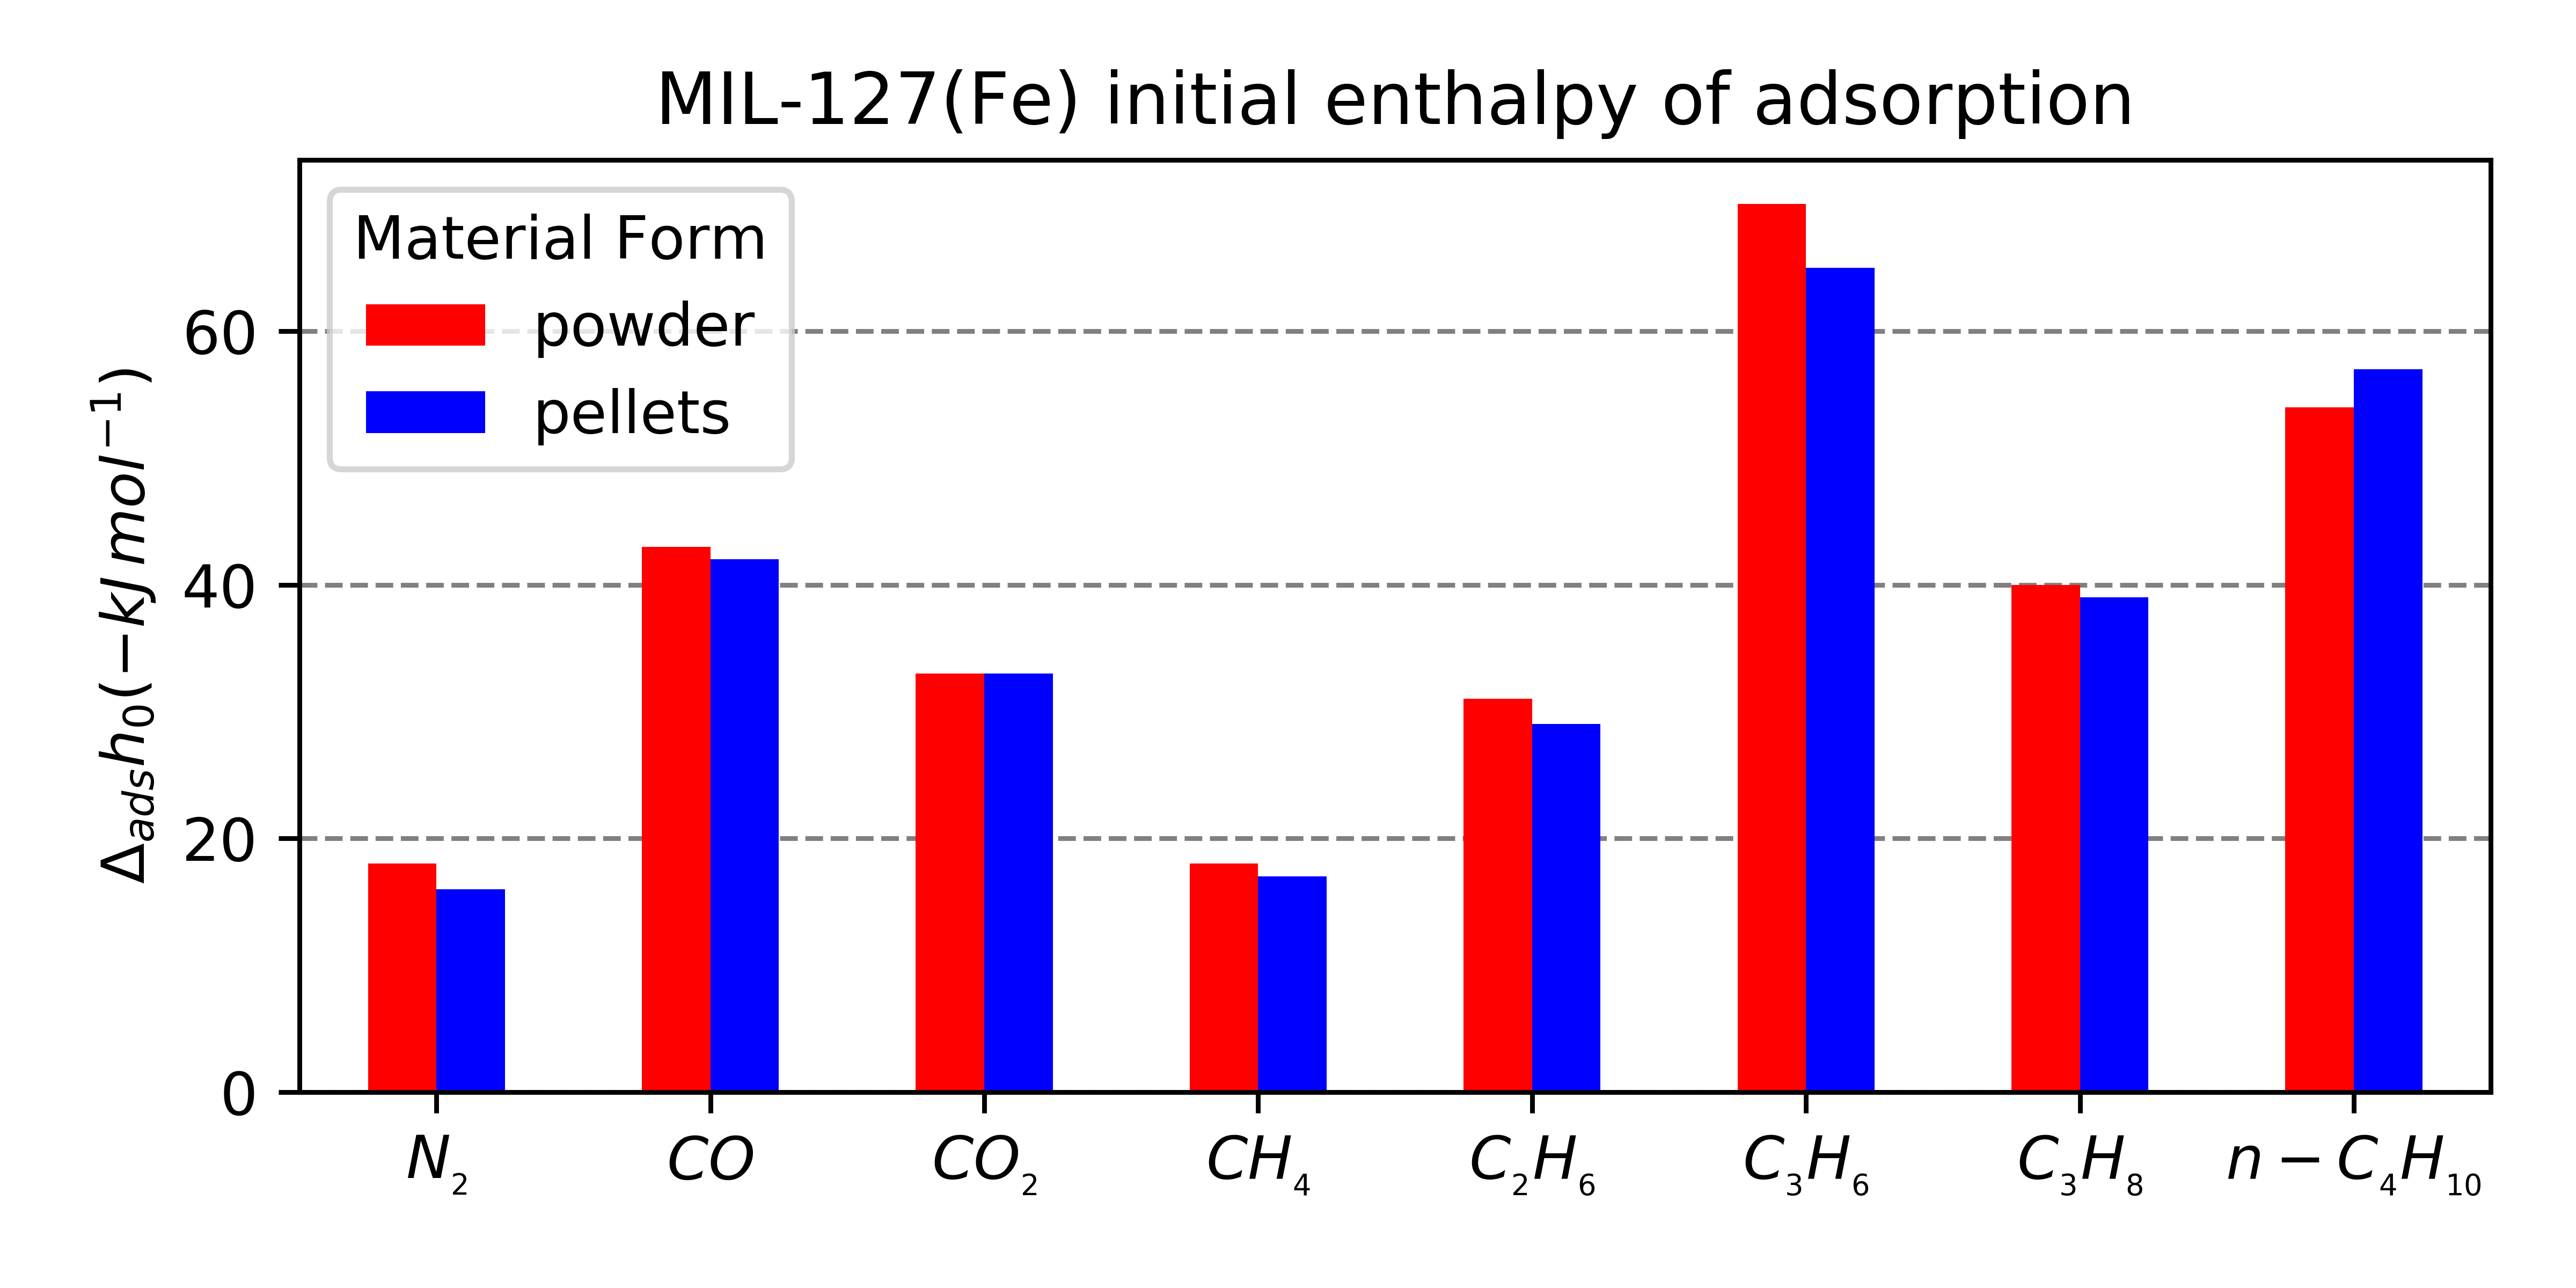
\includegraphics[width=\textwidth]{MIL-127(Fe)-enthalpy-distribution}%
        }%
    \end{subfigure}

    \begin{subfigure}{0.8\textwidth}
        \parbox[c]{0.1\linewidth}{\caption{}\label{fig:analysismil127basis}}%
        \parbox[b]{0.7\linewidth}{%
        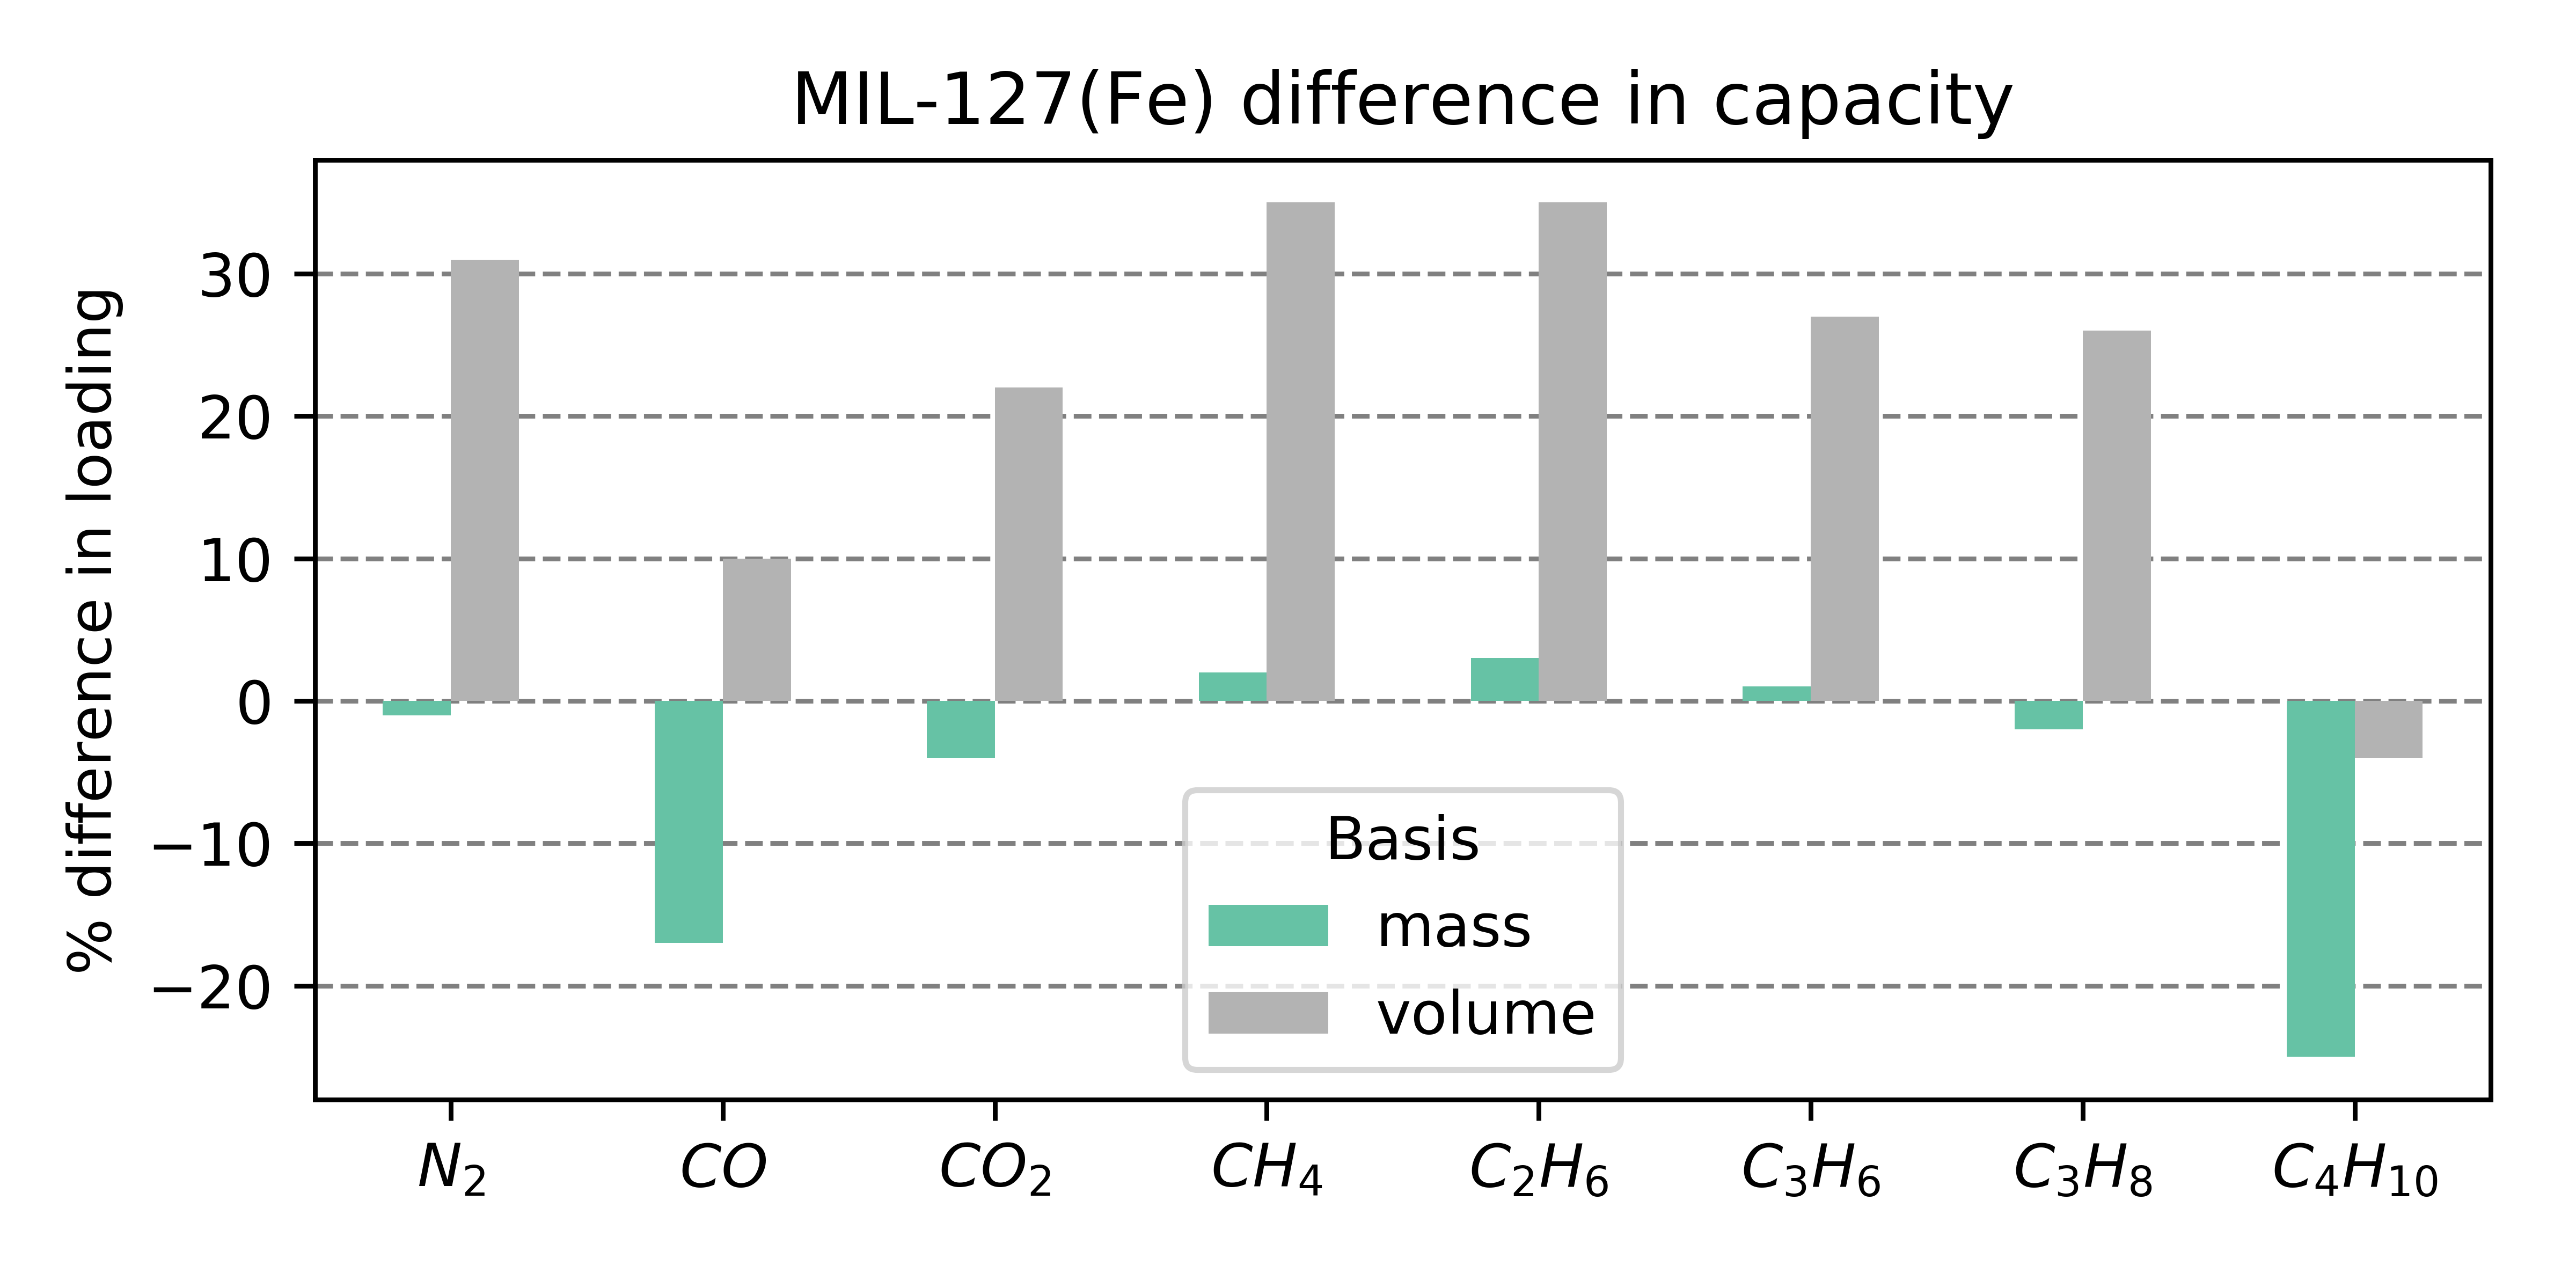
\includegraphics[width=\textwidth]{MIL-127(Fe)-mass-volume}%
        }%
    \end{subfigure}
    
    \caption{MIL-127(Fe) analysis}%
    \label{fig:analysismil127}
\end{figure}